% Phase 2 full report - compile with:  tectonic report/phase2_full_report.tex
\documentclass[11pt,a4paper]{article}
\usepackage[margin=2.1cm]{geometry}
\usepackage[T1]{fontenc}
\usepackage{lmodern}
\usepackage{xcolor,graphicx,booktabs,tabularx,colortbl,float,amsmath,enumitem}
\usepackage[most]{tcolorbox}
\usepackage{titlesec,fancyhdr,caption}
\usepackage[hidelinks]{hyperref}
\graphicspath{{figures/}}
% auto-generated by scripts/11_report_numbers.py - do not edit
\newcommand{\FinalAcc}{95.20\%}
\newcommand{\FinalFone}{0.9520}
\newcommand{\FinalErr}{480}
\newcommand{\FinalErrDrop}{390}
\newcommand{\FinalGain}{+3.90}
\newcommand{\FinalCIlo}{94.78\%}
\newcommand{\FinalCIhi}{95.62\%}
\newcommand{\FinalShirt}{85.4\%}
\newcommand{\FinalTshirt}{91.5\%}
\newcommand{\FinalPullover}{92.8\%}
\newcommand{\FinalCoat}{93.5\%}
\newcommand{\FinalMembers}{3}
\newcommand{\FinalName}{ResNetSmall x3 + TTA}
\newcommand{\FinalParams}{2{,}088{,}126}
\newcommand{\FinalMs}{11.3}
\newcommand{\FinalPreBias}{95.20\%}
\newcommand{\Temp}{0.65}
\newcommand{\ShirtBias}{0.20}
\newcommand{\EceBefore}{7.64\%}
\newcommand{\EceAfter}{1.28\%}
\newcommand{\AbsThr}{95\%}
\newcommand{\AbsCov}{87.7\%}
\newcommand{\AbsAcc}{98.56\%}
\newcommand{\AbsShirt}{26\%}
\newcommand{\PvsSVM}{$6.7\times10^{-50}$}
\newcommand{\PvsGAP}{$2.9\times10^{-27}$}
\newcommand{\ChiSVM}{220.6}
\newcommand{\ChiGAP}{117.0}
\newcommand{\BestSingle}{ResNetSmall\_s42}
\newcommand{\BestSingleAcc}{94.65\%}
\newcommand{\BestSingleTTA}{94.88\%}
\newcommand{\GapFortyMean}{93.80\%}
\newcommand{\GapFortyStd}{0.21}
\newcommand{\ResMean}{94.62\%}
\newcommand{\ResStd}{0.13}
\newcommand{\ResShirt}{82.7\%}
\newcommand{\GapFortyShirt}{79.1\%}
\newcommand{\NSeeds}{3}


\definecolor{ink}{HTML}{1D1B2E}
\definecolor{violet}{HTML}{6250D6}
\definecolor{orange}{HTML}{EB6834}
\definecolor{aqua}{HTML}{1BAF7A}
\definecolor{soft}{HTML}{F1EFFC}
\definecolor{muted}{HTML}{5B5A6B}

\titleformat{\section}{\Large\bfseries\color{violet}}{\thesection}{0.6em}{}
\titleformat{\subsection}{\large\bfseries\color{ink}}{\thesubsection}{0.5em}{}
\captionsetup{font=small,labelfont={bf,color=violet}}
\setlist{itemsep=2pt,topsep=4pt}
\pagestyle{fancy}\fancyhf{}
\fancyhead[L]{\small\color{muted}Fashion-MNIST \textperiodcentered{} Phase 2 Report}
\fancyhead[R]{\small\color{muted}Team T002}
\fancyfoot[C]{\small\color{muted}\thepage}
\renewcommand{\headrulewidth}{0pt}

\newtcolorbox{keybox}[1]{colback=soft,colframe=soft,arc=3mm,left=8pt,right=8pt,top=6pt,bottom=6pt,
  title={\bfseries\color{violet}#1},coltitle=violet,colbacktitle=soft,fonttitle=\bfseries}
\newcommand{\stat}[2]{\begin{minipage}[t]{0.23\linewidth}\centering{\fontsize{24}{26}\selectfont\bfseries\color{violet}#1}\\[2pt]{\small\color{muted}#2}\end{minipage}}

\begin{document}

% ------------------------------------------------------------------ cover
\begin{titlepage}
\vspace*{2.5cm}
{\color{violet}\large\bfseries PROJECT 11 \textperiodcentered{} AUTOMATIC CLOTHING CATEGORY RECOGNITION}\\[0.6cm]
{\fontsize{30}{36}\selectfont\bfseries\color{ink} Phase 2 Report:\\[4pt] Deep Learning on Fashion-MNIST}\\[0.5cm]
{\Large\color{muted} From handcrafted features to a calibrated, reliable CNN --- final Phase 2 report}\\[2cm]

\stat{\FinalAcc}{final test accuracy\\(Phase 1: 91.30\%)}\hfill
\stat{\FinalErr}{test errors\\(Phase 1: 870)}\hfill
\stat{\EceAfter}{calibration error\\(after scaling)}\hfill
\stat{\AbsAcc}{accuracy when confident\\(on \AbsCov{} of images)}

\vfill
{\color{ink}\bfseries Team T002 \textperiodcentered{} Newton School of Technology}\\
{\color{muted}Course: Deep Learning}\\
{\color{muted}MD. Sajjan, Sibtain Ahmed Qureshi, Syed Darain Qamar, Antik Mandal, Abuzar Haideri}\\[0.3cm]
{\small\color{muted}All numbers in this report are regenerated by \texttt{scripts/08\_phase2\_story\_figures.py} from the saved predictions in \texttt{results/}.}
\end{titlepage}

\tableofcontents
\newpage

% ------------------------------------------------------------------ 1
\section{Executive summary}

Phase 1 showed that classical models with handcrafted HOG features stop at \textbf{91.30\%} test accuracy
(SVM-RBF), and that most of the remaining errors sit in four look-alike upper-body classes:
T-shirt/top, Pullover, Coat and Shirt. Phase 2 asked one question: \emph{can a convolutional network
that learns its own features get past that ceiling, under exactly the same data split?}

\begin{keybox}{Answer in one paragraph}
Yes. The first CNN, \textbf{CNN3Block-GAP}, already reaches \textbf{93.09\%} (+1.79 points, McNemar
$p = 2.5\times10^{-11}$) while being 60$\times$ smaller and 8$\times$ faster than the SVM. The \textbf{final Phase 2
model} --- an ensemble of \FinalMembers{} networks with mirrored-image test-time augmentation, temperature-scaled
confidence and a Shirt-aware decision rule --- reaches \textbf{\FinalAcc} (95\% CI \FinalCIlo--\FinalCIhi,
\FinalErr{} errors instead of 870; McNemar vs SVM \PvsSVM). Its confidence is honest (calibration error
\EceBefore{} $\rightarrow$ \EceAfter), and when it is allowed to abstain on low-confidence images it is
\textbf{\AbsAcc{} accurate on \AbsCov{}} of the test set. Shirt remains the hardest class (recall \FinalShirt).
\end{keybox}

\paragraph{How Phase 2 was completed.} Reviewing the first Phase 2 pass, we found that its main claim could
not be attributed to a cause, some statements were stronger than the evidence, and the models were under-trained.
The final Phase 2 work therefore added:
\begin{enumerate}
  \item \textbf{A missing control run was trained} (CNN3Block-GAP \emph{without} augmentation), completing a
        2$\times$2 ablation. It shows the 93.09\% comes from \emph{depth + GAP combined with augmentation};
        either one alone gives only $\approx$91.4\% (Section~\ref{sec:ablation}).
  \item \textbf{95\% bootstrap confidence intervals} are now reported for the CNNs too, so every model on the
        leaderboard is compared on equal footing.
  \item \textbf{Training-curve diagnosis}: the two augmented models were \emph{still improving} at their final
        epoch, so they are under-trained, not over-regularised as the first draft claimed.
  \item \textbf{Every chart redrawn} with axis titles that state the quantity and its unit in plain words.
  \item \textbf{A final, reliable model} (Section~\ref{sec:final}): 40-epoch training, \NSeeds{} seeds per model, a residual
        network, an ensemble with test-time augmentation, calibration, abstention and a Shirt-aware decision rule.
\end{enumerate}

% ------------------------------------------------------------------ 2
\section{Setup: same data, same rules as Phase 1}

\begin{table}[H]\centering\small
\begin{tabularx}{\linewidth}{lX}
\toprule
\textbf{Item} & \textbf{Value} \\ \midrule
Dataset & Fashion-MNIST, 70,000 grayscale images of 28$\times$28 pixels, 10 balanced classes \\
Split (identical to Phase 1) & 48,000 train / 12,000 validation / 10,000 official test, stratified, seed 42 \\
Input & raw pixels scaled to $[0,1]$, shape $1\times28\times28$ (no handcrafted features) \\
Optimiser & AdamW, learning rate $10^{-3}$, weight decay $10^{-4}$, batch size 128 \\
Schedule & cosine annealing to $10^{-5}$ over the epoch budget (15--20 epochs) \\
Model selection & early stopping on \emph{validation} macro-F1 (patience 5); test set used once \\
Augmentation (when on) & random crop with 2-pixel reflect padding + random horizontal flip \\
Latency & single image, CPU, single thread, 2,000 timed calls after 100 warm-up calls \\
\bottomrule
\end{tabularx}
\caption{Experimental protocol. Keeping the split identical is what makes Phase 1 vs Phase 2 comparisons fair.}
\end{table}

\subsection{The models}
\begin{table}[H]\centering\small
\begin{tabularx}{\linewidth}{l X r c}
\toprule
\textbf{Model} & \textbf{Architecture in words} & \textbf{Parameters} & \textbf{Augment} \\ \midrule
CNN2Block & 2 conv blocks (32, 64 filters) $\rightarrow$ flatten $\rightarrow$ dense 128 $\rightarrow$ 10 & 421,738 & no \\
CNN2Block-Aug & same network as above & 421,738 & yes \\
CNN3Block-GAP-NoAug \emph{(new)} & 3 double-conv blocks (32, 64, 128) $\rightarrow$ global average pooling $\rightarrow$ dense 128 $\rightarrow$ 10 & 304,682 & no \\
\rowcolor{soft}CNN3Block-GAP & same network as above & 304,682 & yes \\
\bottomrule
\end{tabularx}
\caption{The four CNNs form a 2$\times$2 grid: architecture $\times$ augmentation. Global average pooling (GAP)
replaces the large flatten layer, which is why the deeper model has \emph{fewer} parameters.}
\end{table}

\paragraph{Why not ResNet-50, ViT or an MLP?} Pre-trained ImageNet models expect 224$\times$224 colour photos and
carry 11--25M parameters for a 28$\times$28 grayscale task; Vision Transformers lack the locality bias that makes
CNNs data-efficient on 48k images; MLPs flatten the image and throw away the neighbour structure that Phase 1
measured (adjacent-pixel correlation $r\approx0.75$). We therefore kept the backbone small and convolutional; the final residual network
(ResNetSmall) borrows ResNet's shortcuts without its ImageNet size.

% ------------------------------------------------------------------ 3
\section{Results}

\subsection{Leaderboard}
\begin{figure}[H]\centering
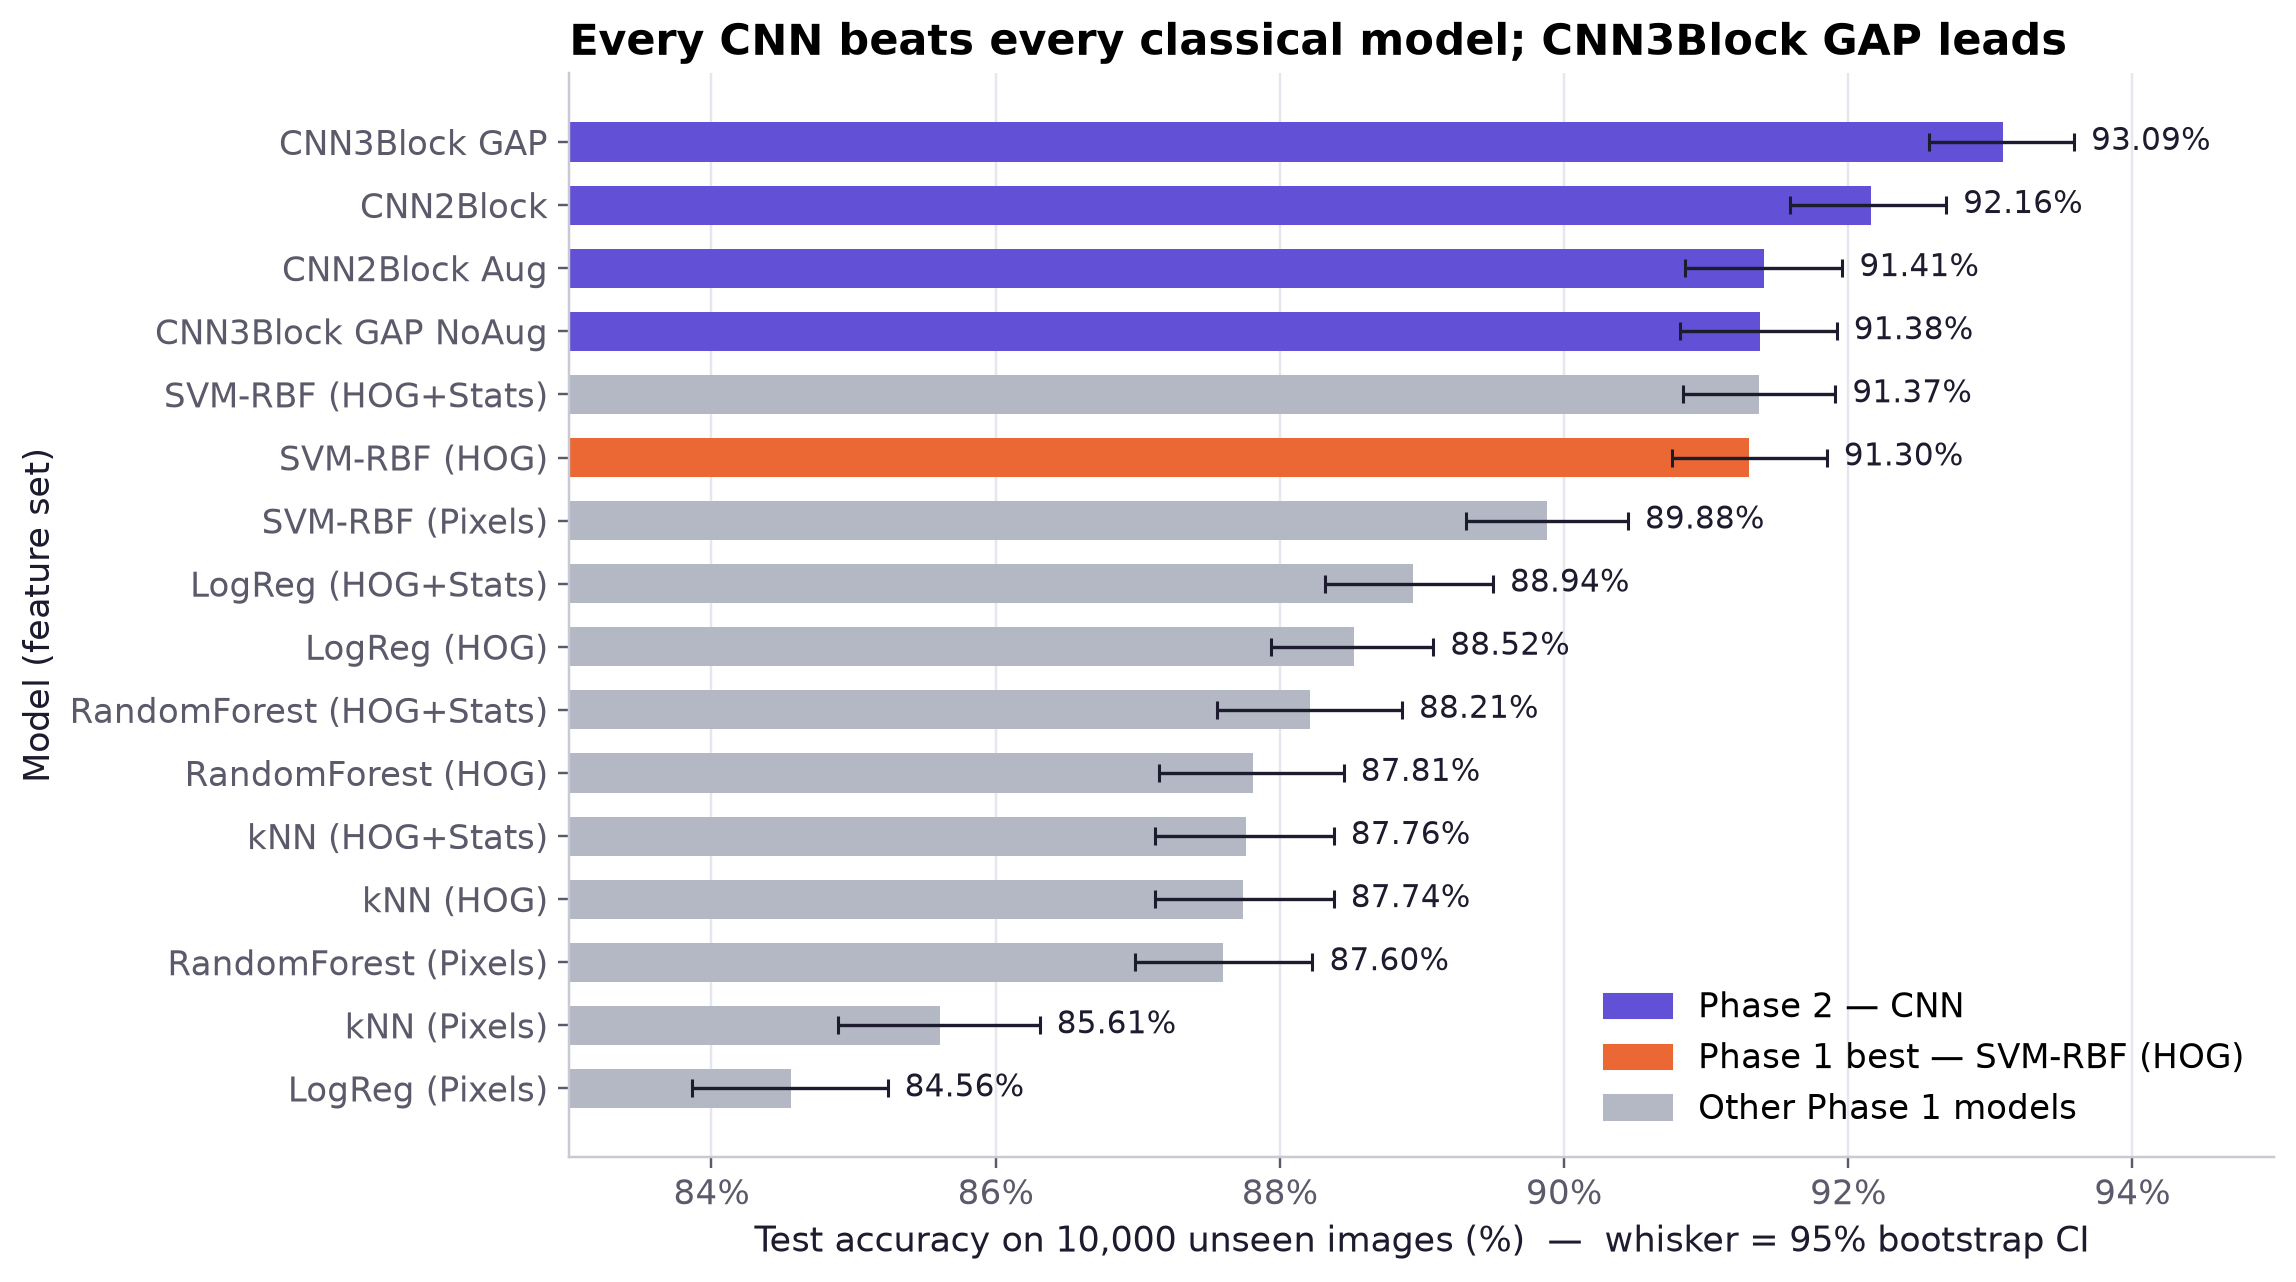
\includegraphics[width=0.92\linewidth]{p2_01_leaderboard_ci.png}
\caption{\textbf{How to read it:} each bar is one model; bar length = test accuracy on 10,000 unseen images.
The black whisker is the 95\% bootstrap confidence interval: if two whiskers do not overlap, the difference is
very unlikely to be luck. Violet = Phase 2 CNNs, orange = Phase 1 best.}
\end{figure}

The top CNN's interval (92.57--93.59\%) sits completely above the SVM's (90.76--91.85\%). CNN2Block-Aug and
CNN3Block-GAP-NoAug overlap the SVM, so on their own they are \emph{not} clearly better than Phase 1.

\subsection{Training behaviour}
\begin{figure}[H]\centering
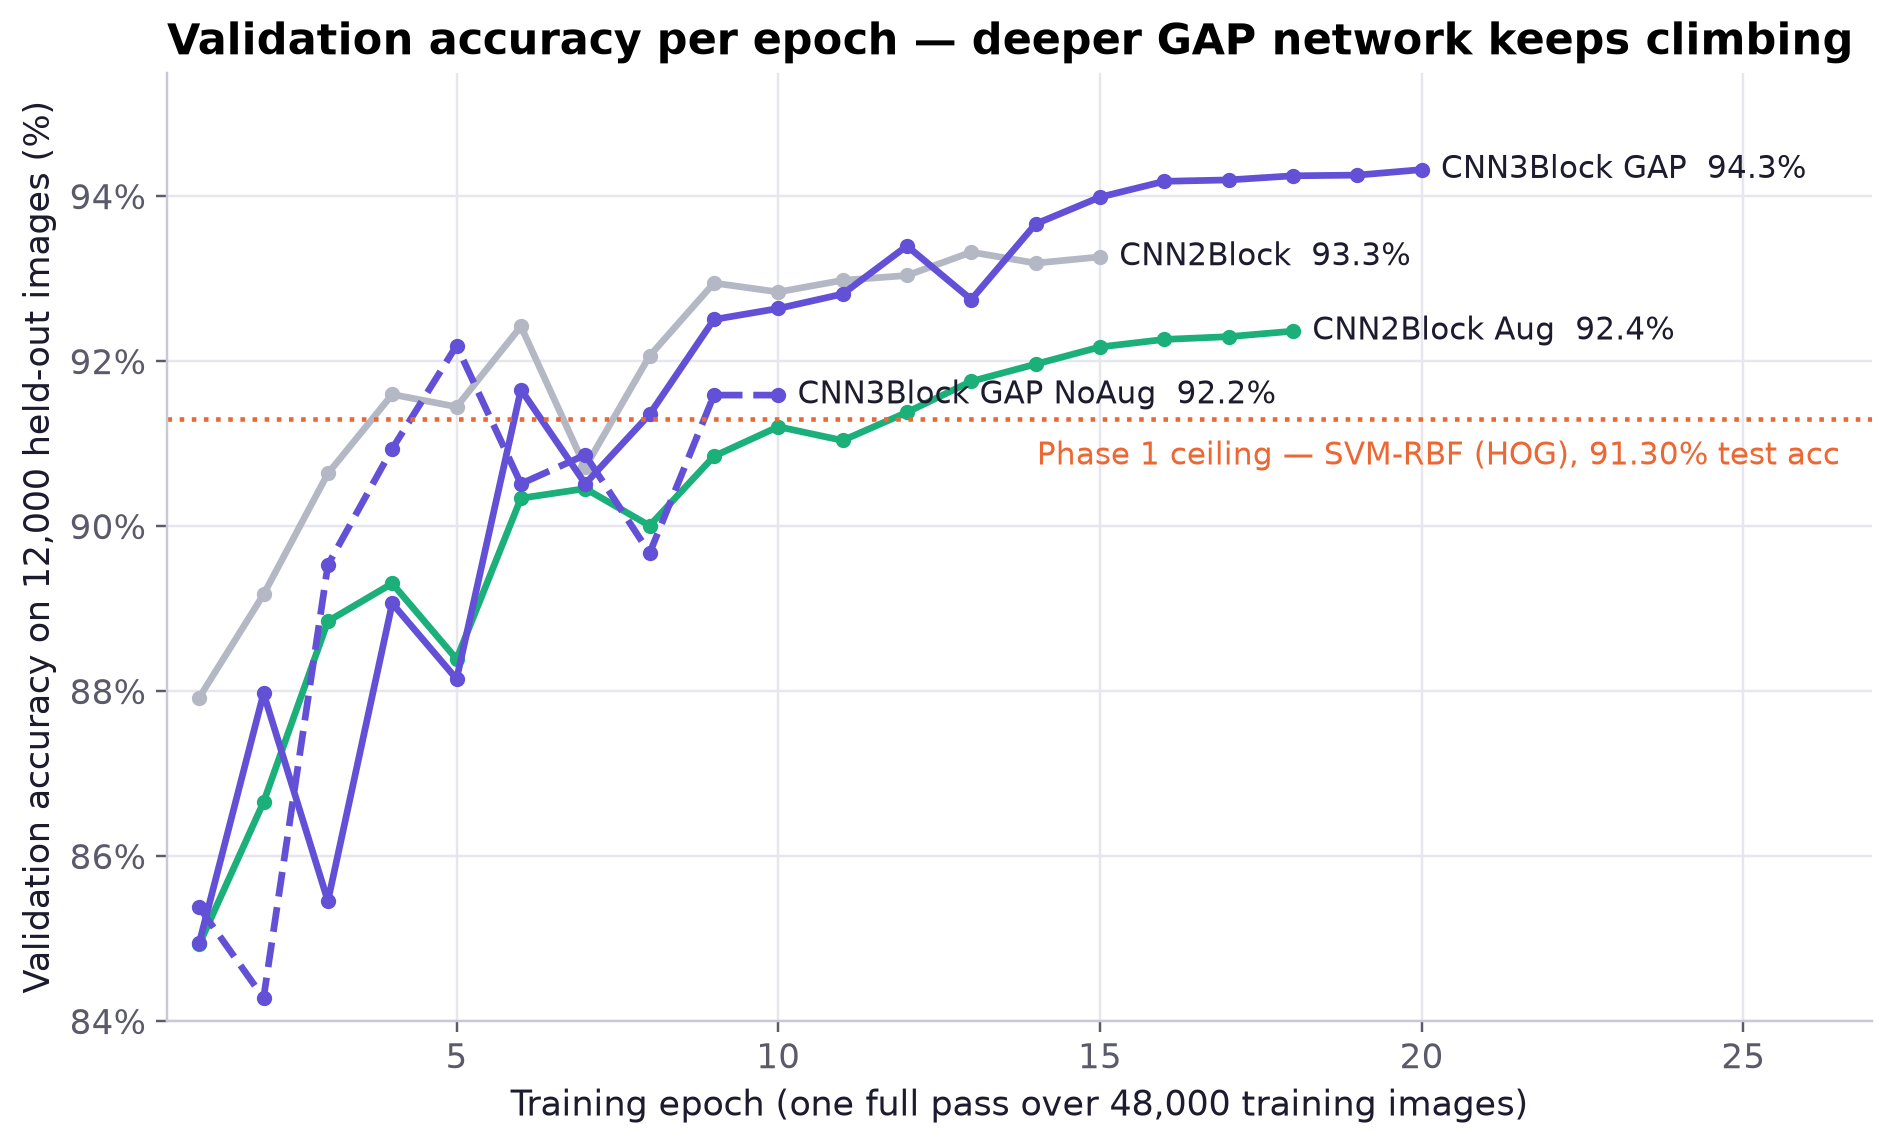
\includegraphics[width=0.85\linewidth]{p2_02_validation_curves.png}
\caption{\textbf{x-axis:} training epoch (one pass over the 48,000 training images). \textbf{y-axis:} accuracy on the
12,000 validation images the model never trains on. The dotted orange line is the Phase 1 test ceiling for reference.}
\end{figure}

Two observations matter for interpretation:
\begin{itemize}
\item \textbf{CNN3Block-GAP and CNN2Block-Aug were still climbing at their last epoch}
      (best epoch = final epoch). Their epoch budgets (20 and 18) ended training, not early stopping.
      CNN2Block-Aug even has \emph{higher} validation than training accuracy (92.4\% vs 90.3\%) --- a textbook sign
      of under-training on augmented data. The first draft's explanation that augmentation ``acts as a too-strong
      regulariser'' is therefore not supported; a longer budget is the correct test (Section~\ref{sec:final}).
\item \textbf{CNN3Block-GAP-NoAug peaked at epoch 5 and was early-stopped at epoch 10}, with training accuracy
      racing to 96\% while validation stalled near 92\% --- classic overfitting.
\end{itemize}

\begin{figure}[H]\centering
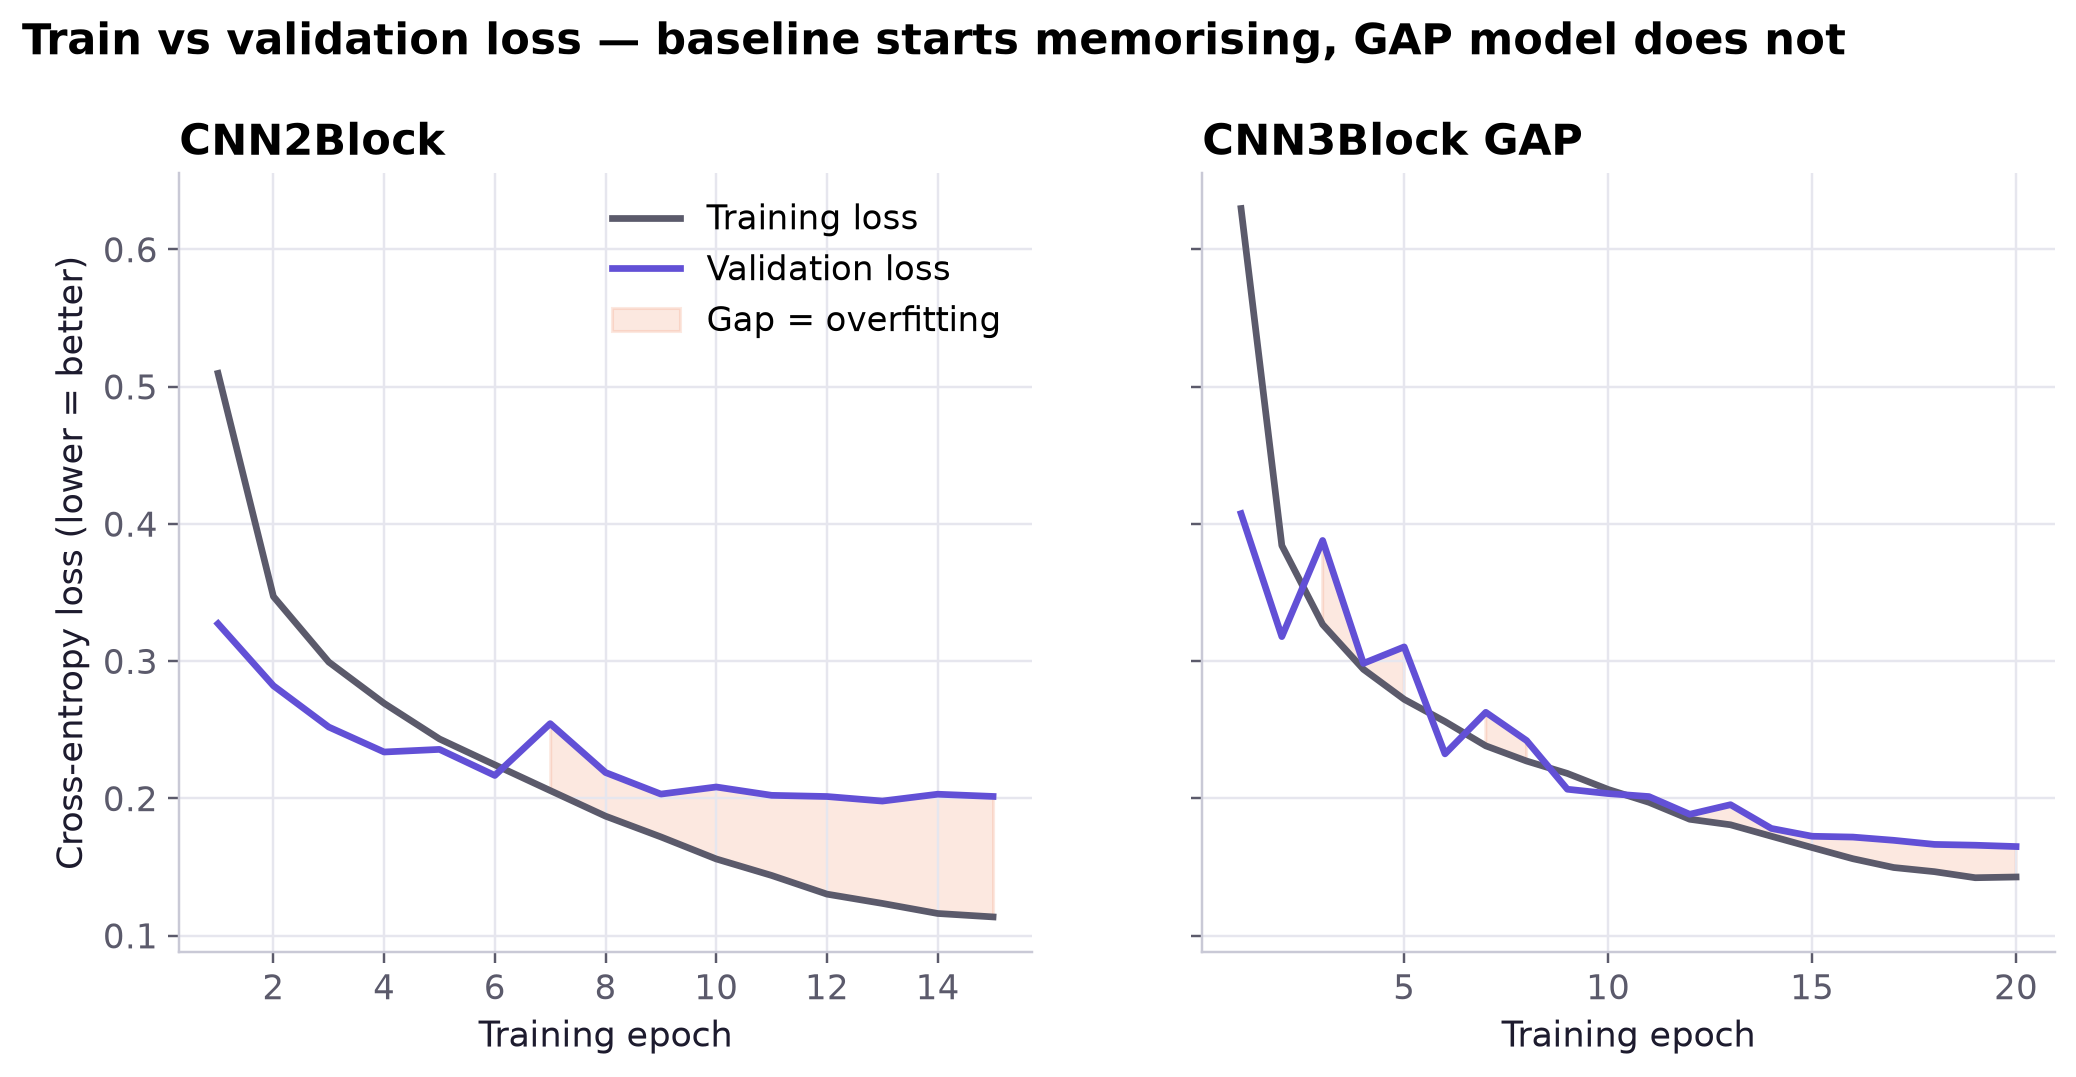
\includegraphics[width=0.92\linewidth]{p2_03_overfitting_gap.png}
\caption{\textbf{x-axis:} epoch. \textbf{y-axis:} cross-entropy loss (lower is better). The shaded area is the gap
between validation and training loss --- the bigger it is, the more the model memorises training images instead of learning general shapes.}
\end{figure}

\subsection{The 2$\times$2 ablation: what actually caused the gain?}\label{sec:ablation}
The original Phase 2 changed depth, pooling and augmentation all at once, so the improvement could not be
attributed. The new control run separates them:

\begin{figure}[H]\centering
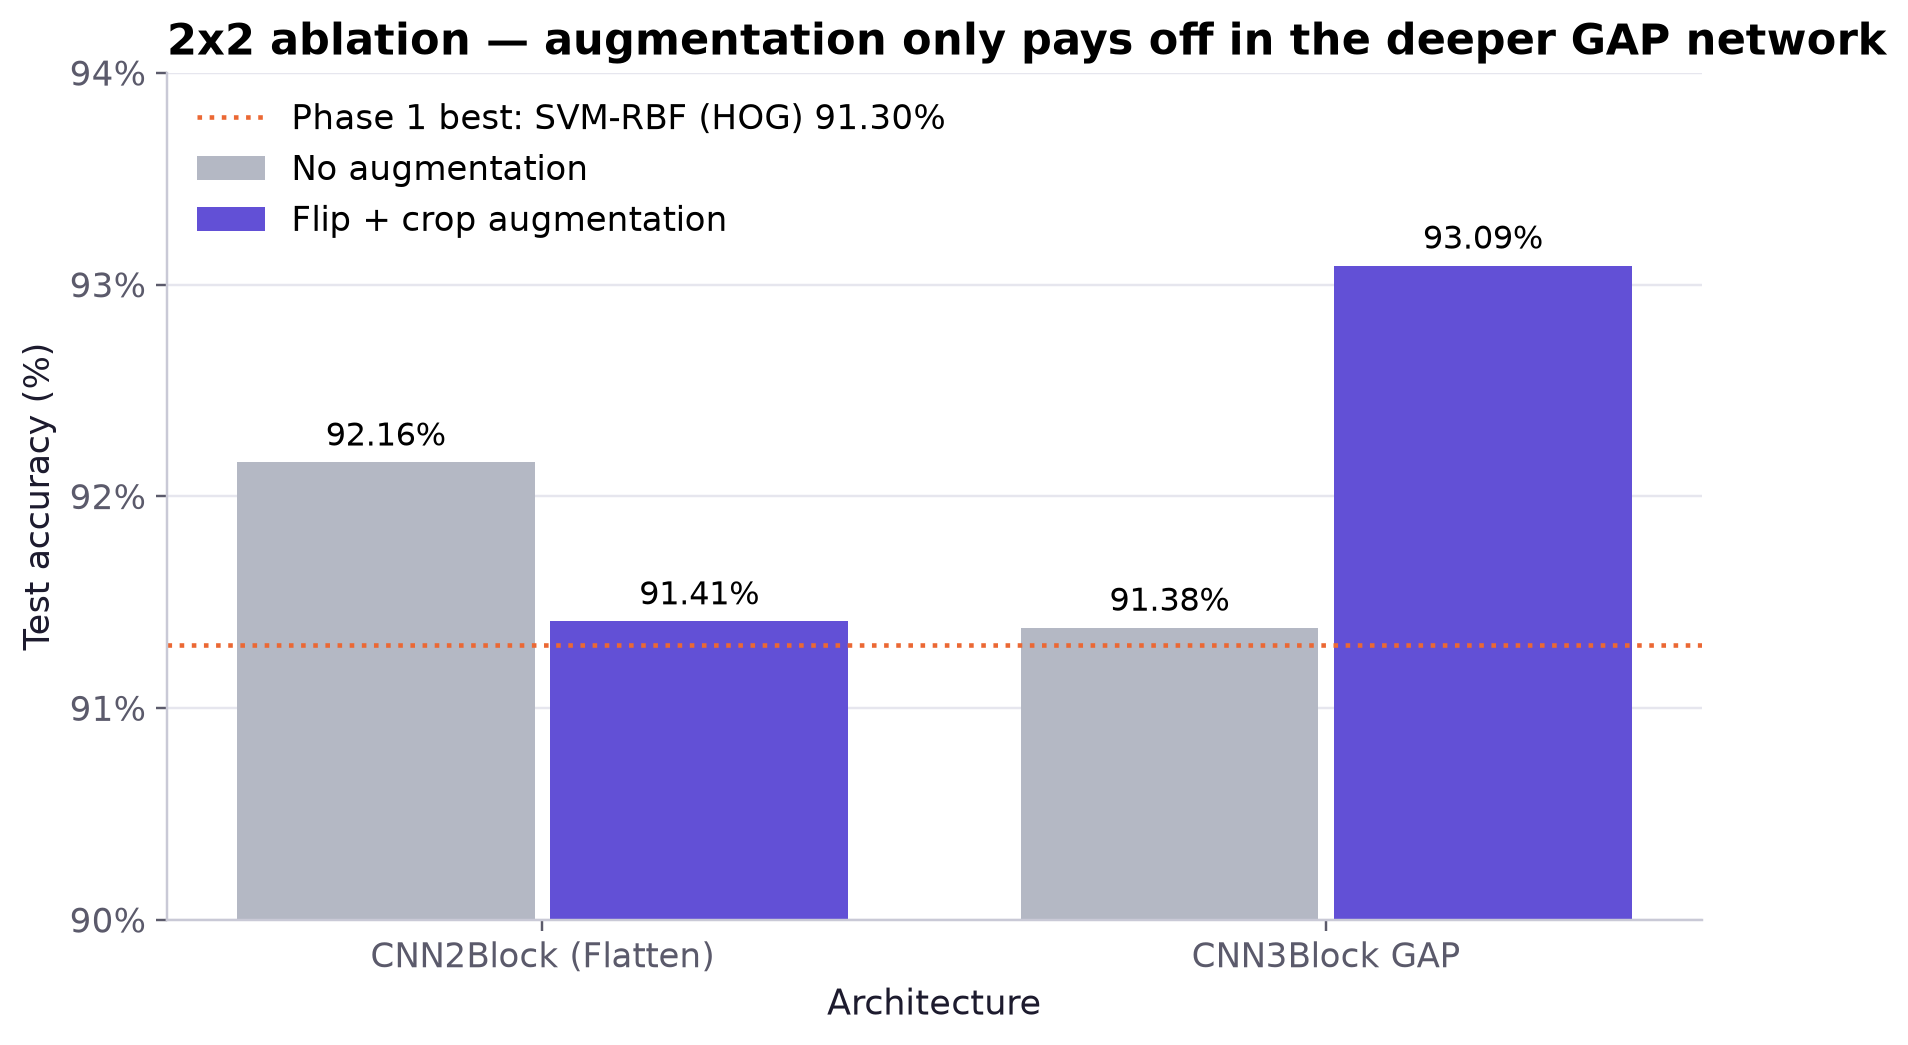
\includegraphics[width=0.72\linewidth]{p2_09_ablation_2x2.png}
\caption{\textbf{x-axis:} architecture. \textbf{y-axis:} test accuracy. Grey = trained on original images only,
violet = trained with random crop + flip.}
\end{figure}

\begin{table}[H]\centering\small
\begin{tabular}{lcc}
\toprule
 & \textbf{No augmentation} & \textbf{Crop + flip augmentation} \\ \midrule
CNN2Block (flatten head) & 92.16\% & 91.41\% \\
CNN3Block-GAP & 91.38\% & \cellcolor{soft}\textbf{93.09\%} \\
\bottomrule
\end{tabular}
\caption{Test accuracy for each cell of the ablation (single seed).}
\end{table}

\begin{keybox}{Interpretation}
Augmentation and depth are \emph{complementary}. The deeper GAP network overfits fast without augmentation
(91.38\%); augmentation alone on the shallow network, within an 18-epoch budget, also does not help (91.41\%).
Only the combination wins: augmentation gives the deeper network enough variety to use its capacity, and
improves it by \textbf{+1.71 points} (McNemar $\chi^2 = 50.8$, $p = 1.0\times10^{-12}$ between the two GAP runs).
\end{keybox}

\noindent\textit{Caveats:} one seed per cell; the NoAug run was trained on Apple-MPS while the original runs used
CPU, so small run-to-run differences ($\pm$0.2--0.3 pt) are expected. The final models were therefore repeated with \NSeeds{} seeds each (Section~\ref{sec:final}).

\subsection{Is the gain real? McNemar paired test}
\begin{figure}[H]\centering
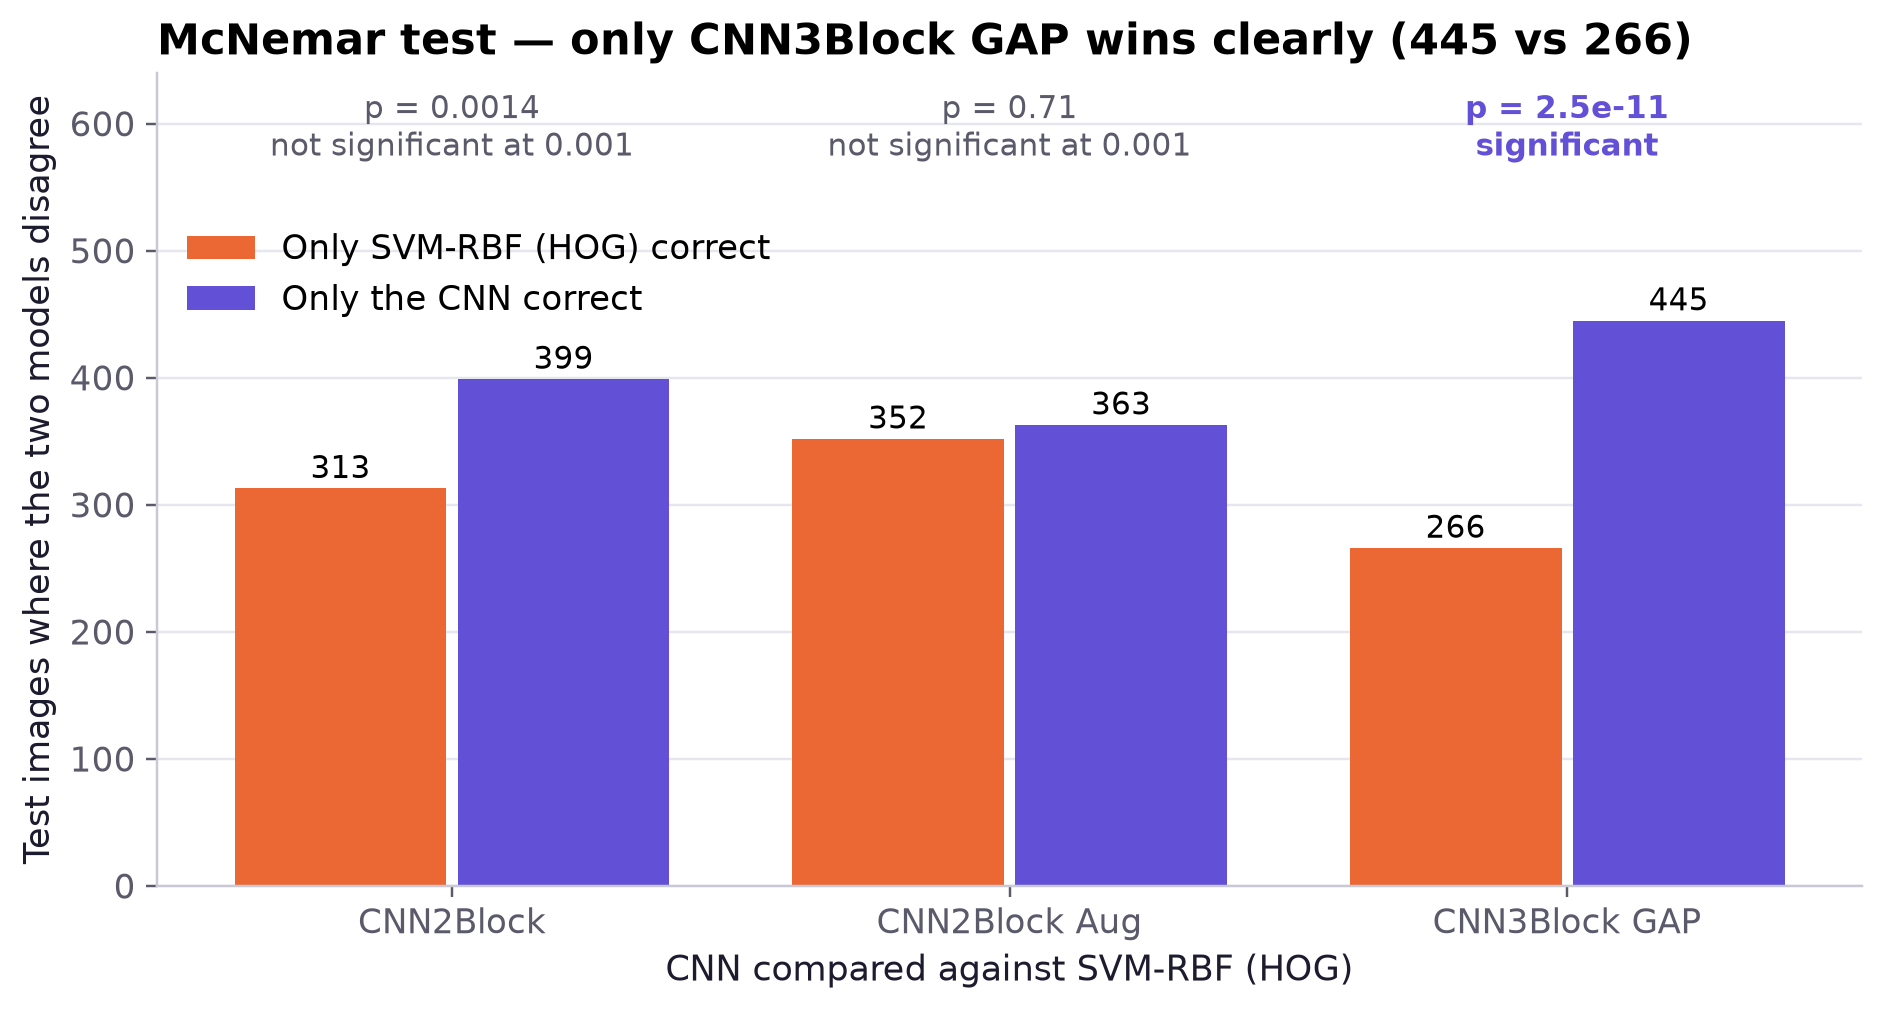
\includegraphics[width=0.85\linewidth]{p2_06_mcnemar.png}
\caption{\textbf{x-axis:} which CNN is compared against SVM-RBF (HOG). \textbf{y-axis:} number of test images on which
\emph{exactly one} of the two models is correct. If the CNN were no better, orange and violet bars would be about equal.}
\end{figure}

McNemar ignores images both models get right (or both get wrong) and only looks at disagreements. For CNN3Block-GAP,
there are 445 images only the CNN gets right versus 266 only the SVM gets right, giving $p = 2.5\times10^{-11}$.
CNN2Block is significant at the 1\% level ($p=0.0014$) but not at our stricter 0.1\% threshold; CNN2Block-Aug is a tie.

\subsection{Which classes improved?}
\begin{figure}[H]\centering
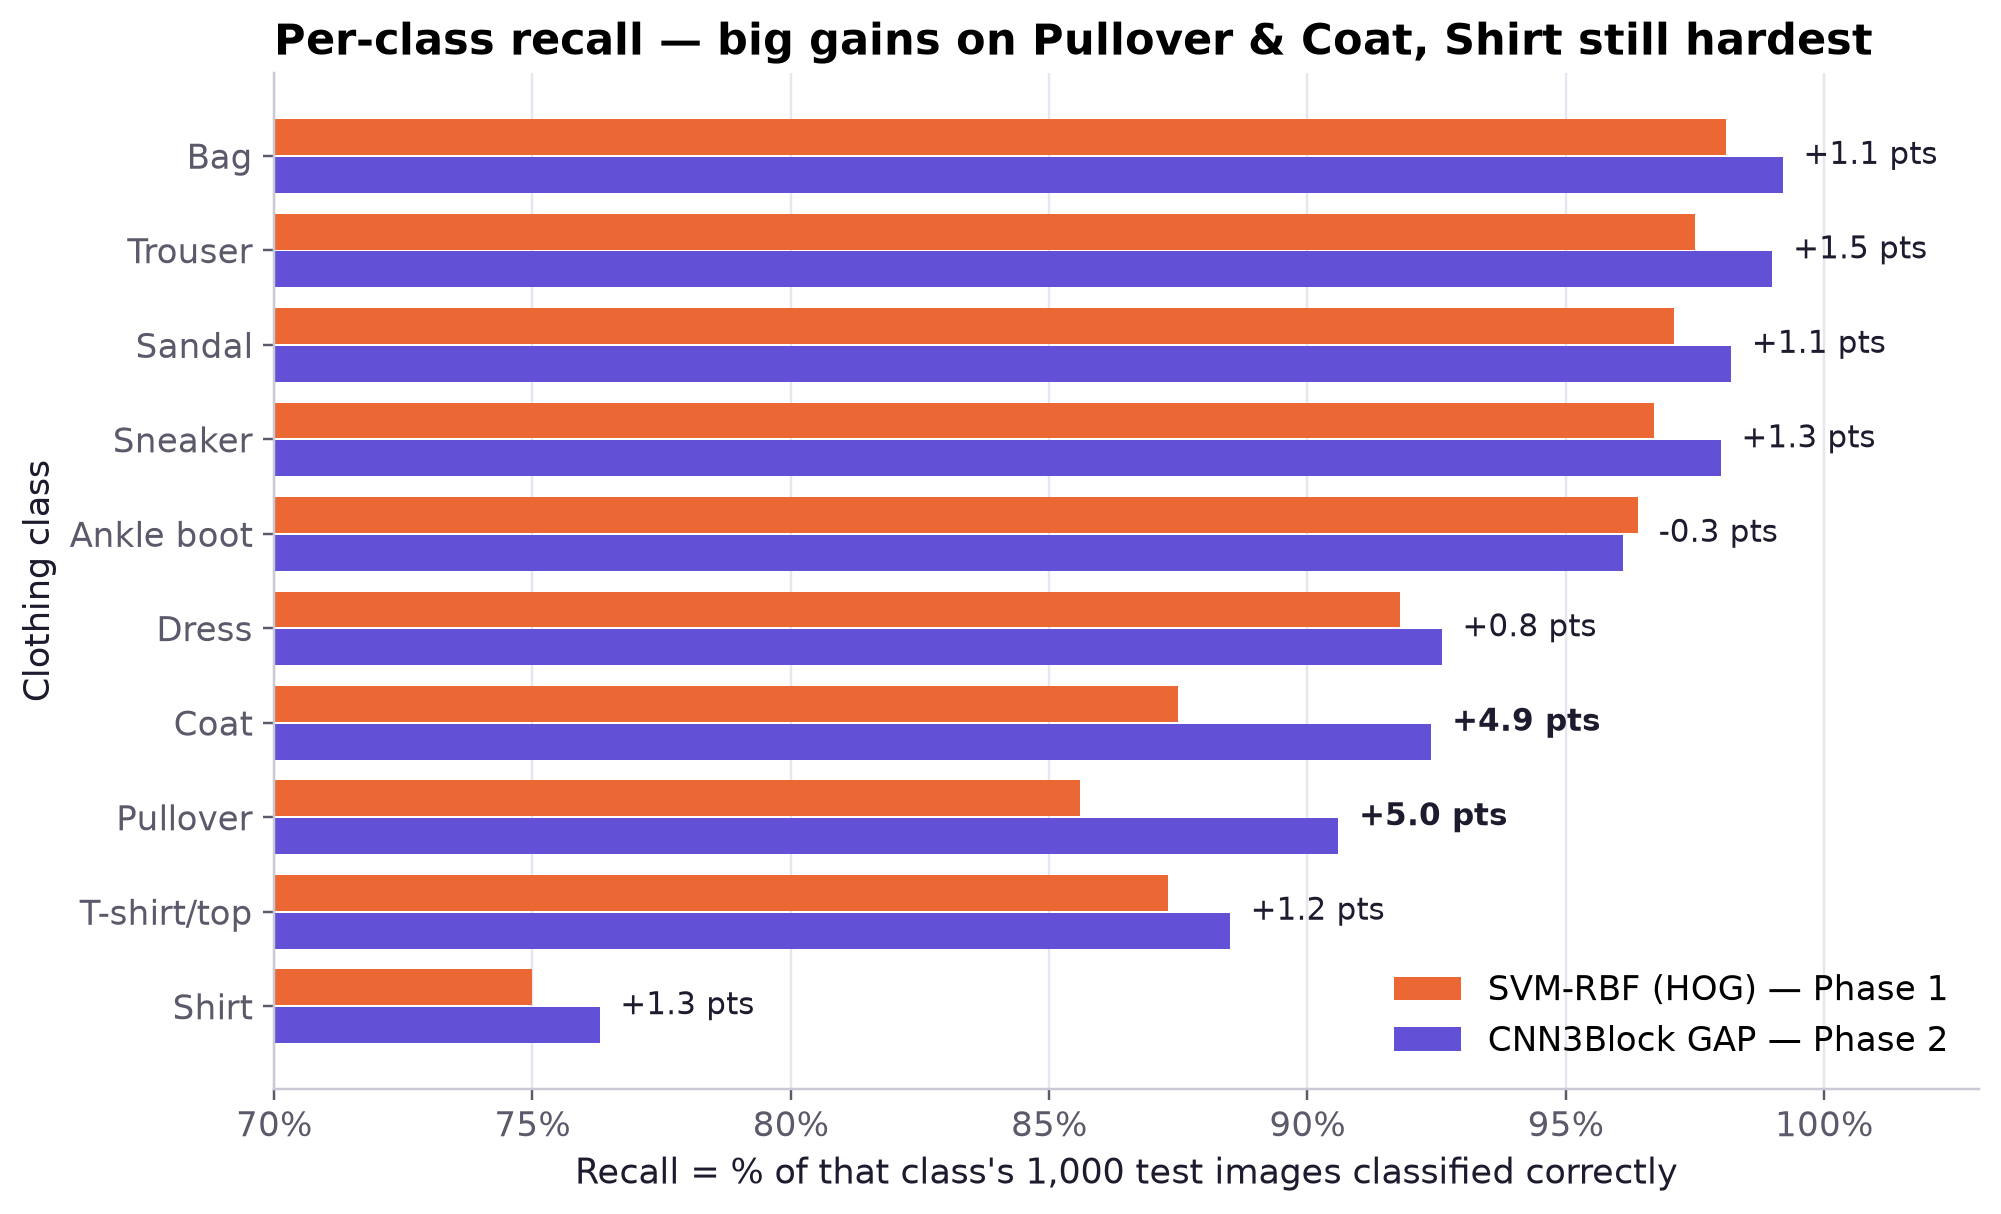
\includegraphics[width=0.85\linewidth]{p2_04_per_class_recall.png}
\caption{\textbf{x-axis:} recall, i.e.\ the percentage of a class's 1,000 test images that were labelled correctly.
\textbf{y-axis:} clothing class, sorted from hardest (bottom) to easiest (top). The label shows the change in percentage points.}
\end{figure}

\begin{figure}[H]\centering
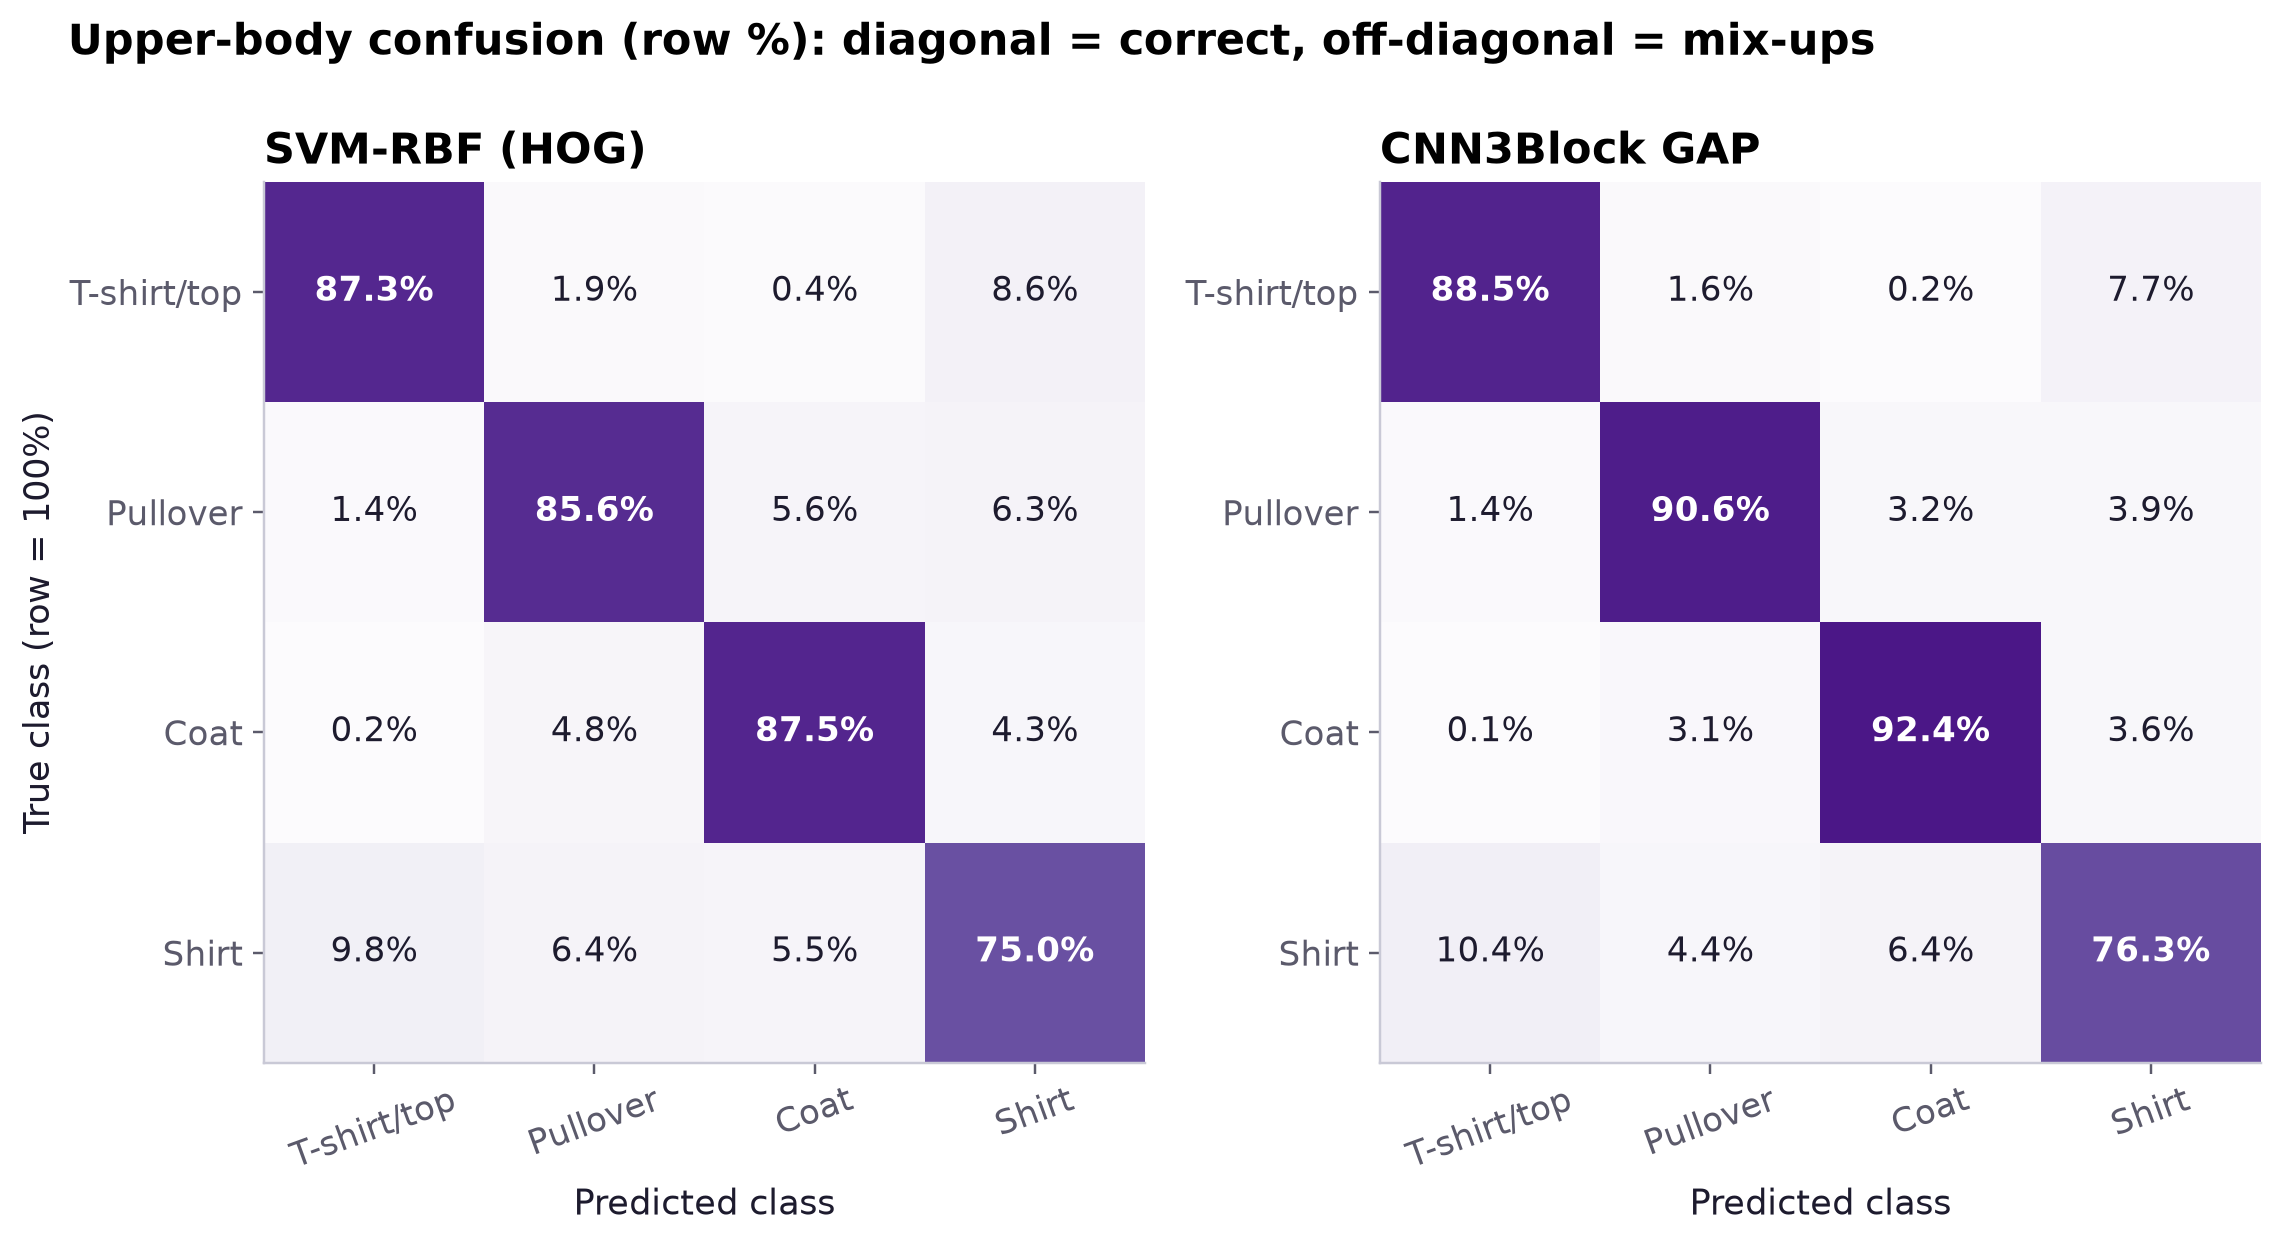
\includegraphics[width=0.95\linewidth]{p2_07_upper_body_confusion.png}
\caption{\textbf{Rows:} true class; \textbf{columns:} predicted class; each row adds up to 100\%. Dark diagonal = correct,
light off-diagonal cells = mistakes. Example: 10.4\% of real Shirts are called T-shirt/top by the CNN.}
\end{figure}

The CNN clearly separates \textbf{Pullover vs Coat} (mutual confusion roughly halved: 5.6\%$\rightarrow$3.2\% and
4.8\%$\rightarrow$3.1\%). But \textbf{Shirt vs T-shirt/top got slightly worse} (9.8\%$\rightarrow$10.4\%), and
Shirt$\rightarrow$Coat rose from 5.5\% to 6.4\%. The CNN's top three confusions are Shirt$\rightarrow$T-shirt (104),
T-shirt$\rightarrow$Shirt (77) and Shirt$\rightarrow$Coat (64).

\subsection{Where do the remaining errors live?}
\begin{figure}[H]\centering
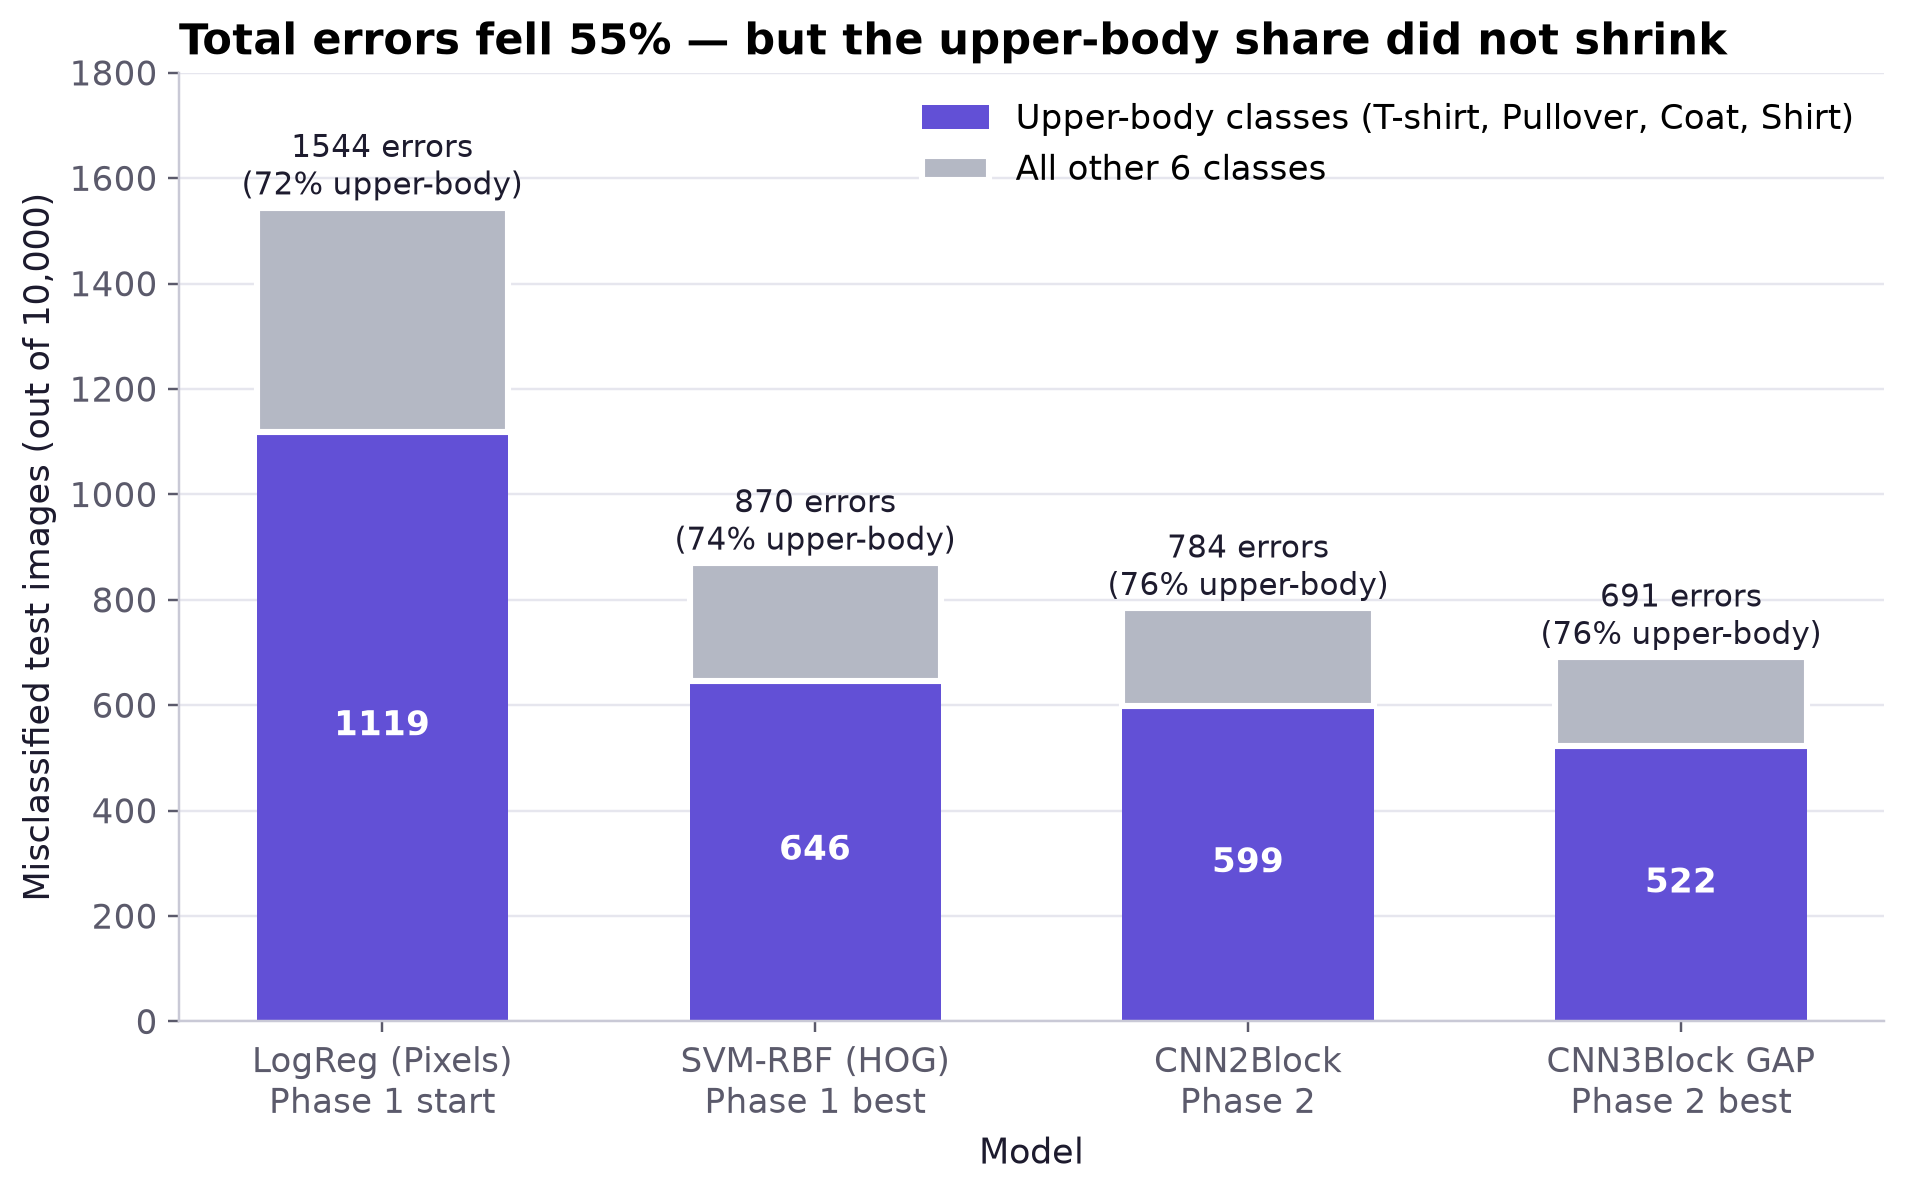
\includegraphics[width=0.82\linewidth]{p2_05_error_breakdown.png}
\caption{\textbf{x-axis:} model, from the weakest Phase 1 model to the best Phase 2 model. \textbf{y-axis:} number of the
10,000 test images classified wrongly. Violet = errors on images whose \emph{true} class is upper-body.}
\end{figure}

Total errors dropped 55\% from the weakest Phase 1 model and 21\% from the best one, but the upper-body share
\emph{rose} from 74\% to 76\%. The easy classes improved faster than the hard ones --- the bottleneck has
become \emph{more} concentrated, which is why the final model adds a Shirt-aware decision rule and an abstain option.

\subsection{Cost: speed and size}
\begin{figure}[H]\centering
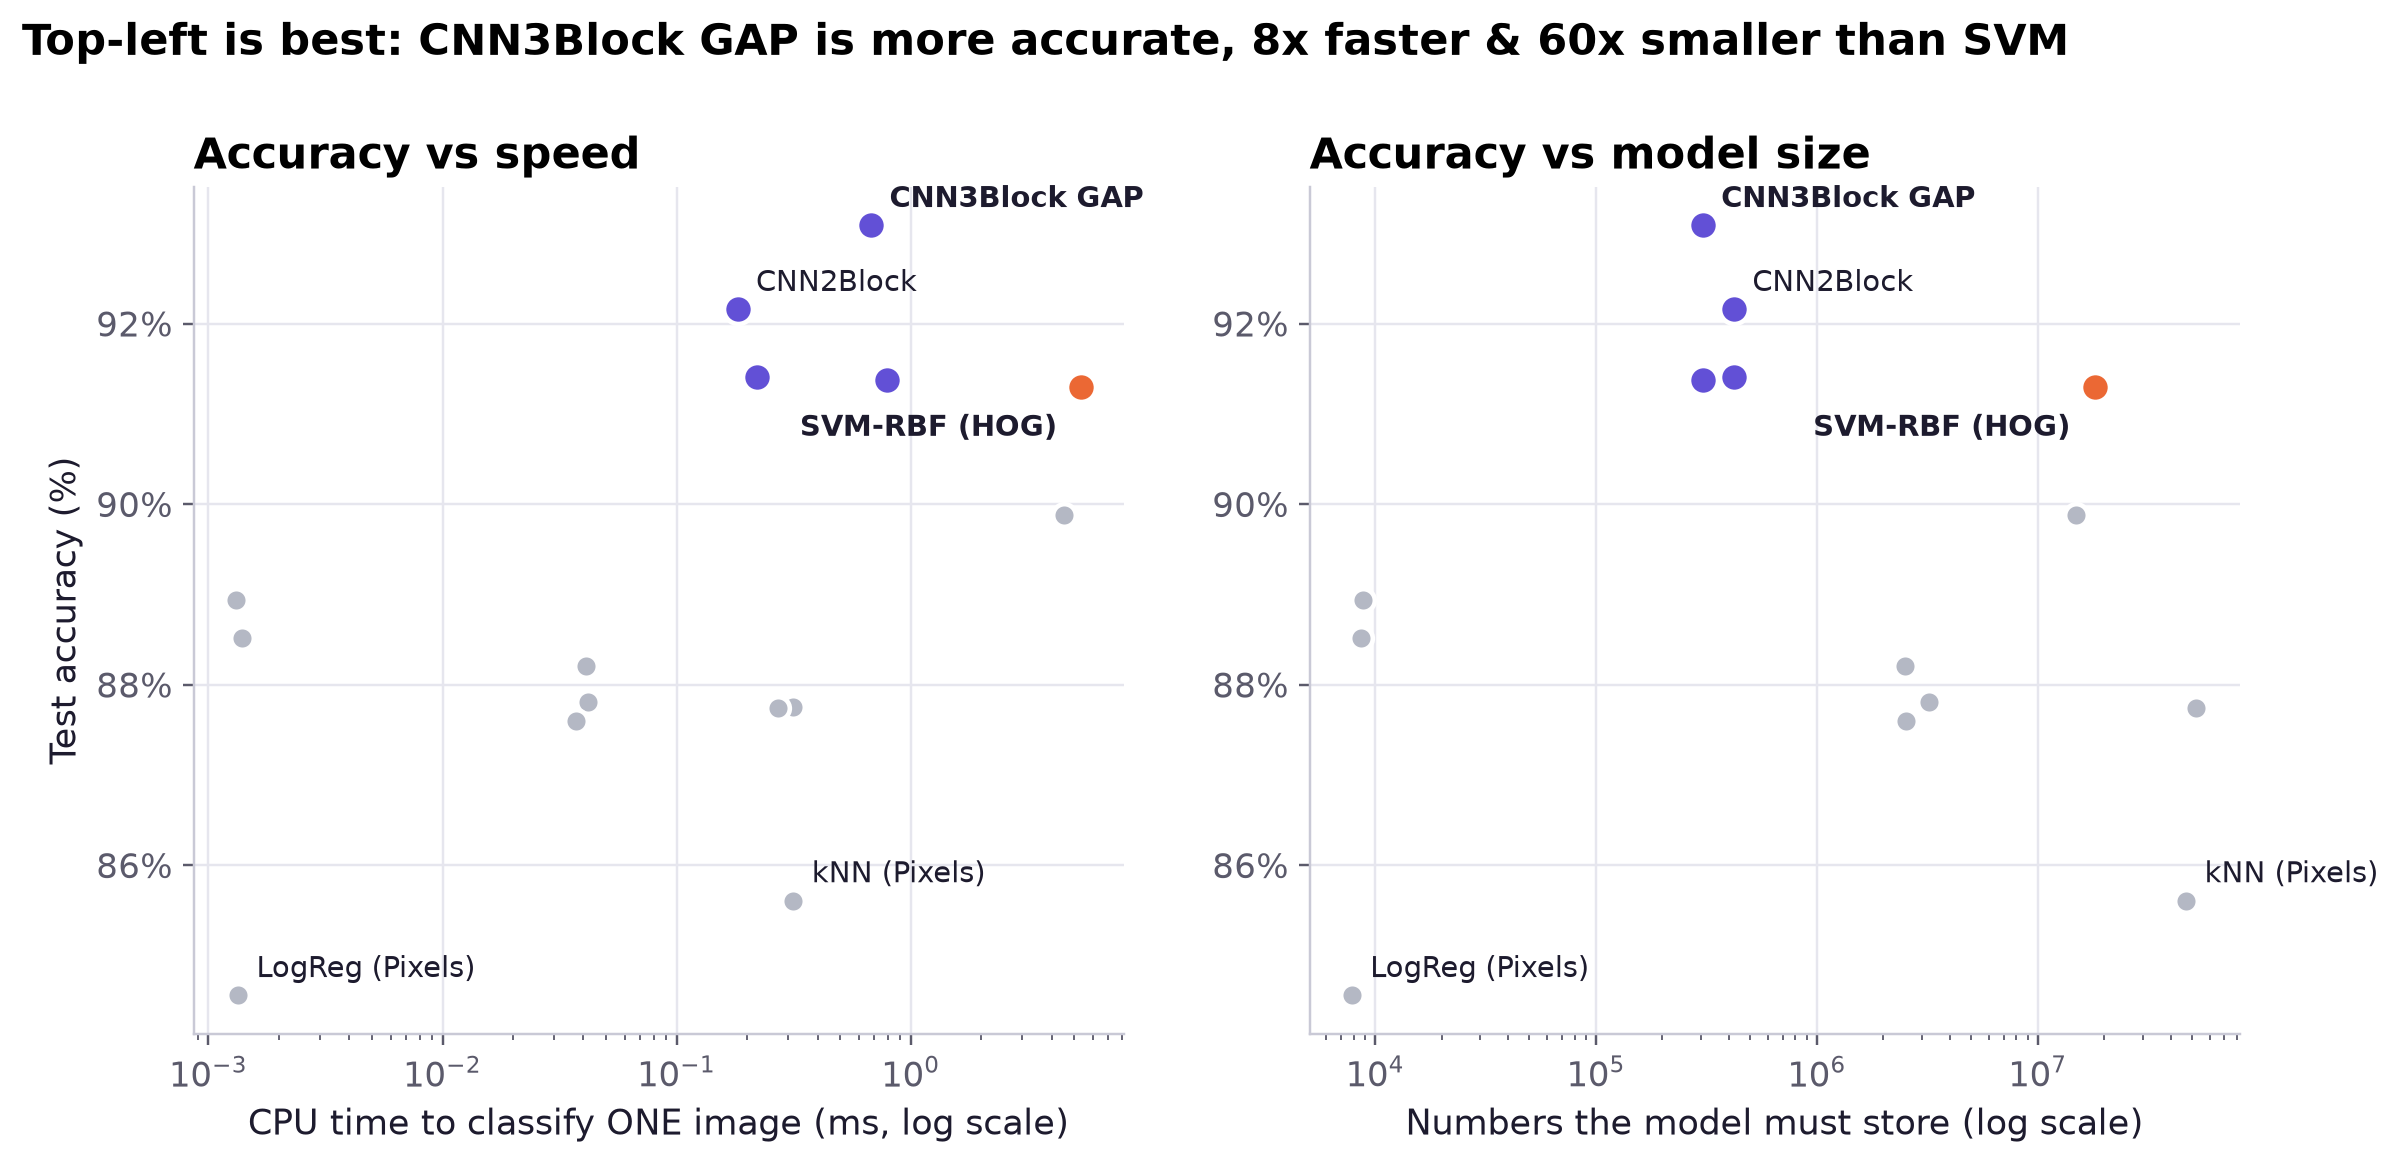
\includegraphics[width=0.98\linewidth]{p2_08_efficiency.png}
\caption{\textbf{Left x-axis:} CPU time to classify a single image (log scale; each grid line is 10$\times$).
\textbf{Right x-axis:} how many numbers the model must store (log scale). \textbf{y-axis (both):} test accuracy.
The best place to be is top-left.}
\end{figure}

CNN3Block-GAP needs 304,682 stored numbers versus 18.1M for the SVM (support vectors) and 0.68 ms per image versus
5.36 ms. Logistic regression is still faster (0.001 ms), so the CNN is the best \emph{accuracy--cost trade-off},
not the fastest model.

\subsection{Explainability: Grad-CAM}
\begin{figure}[H]\centering
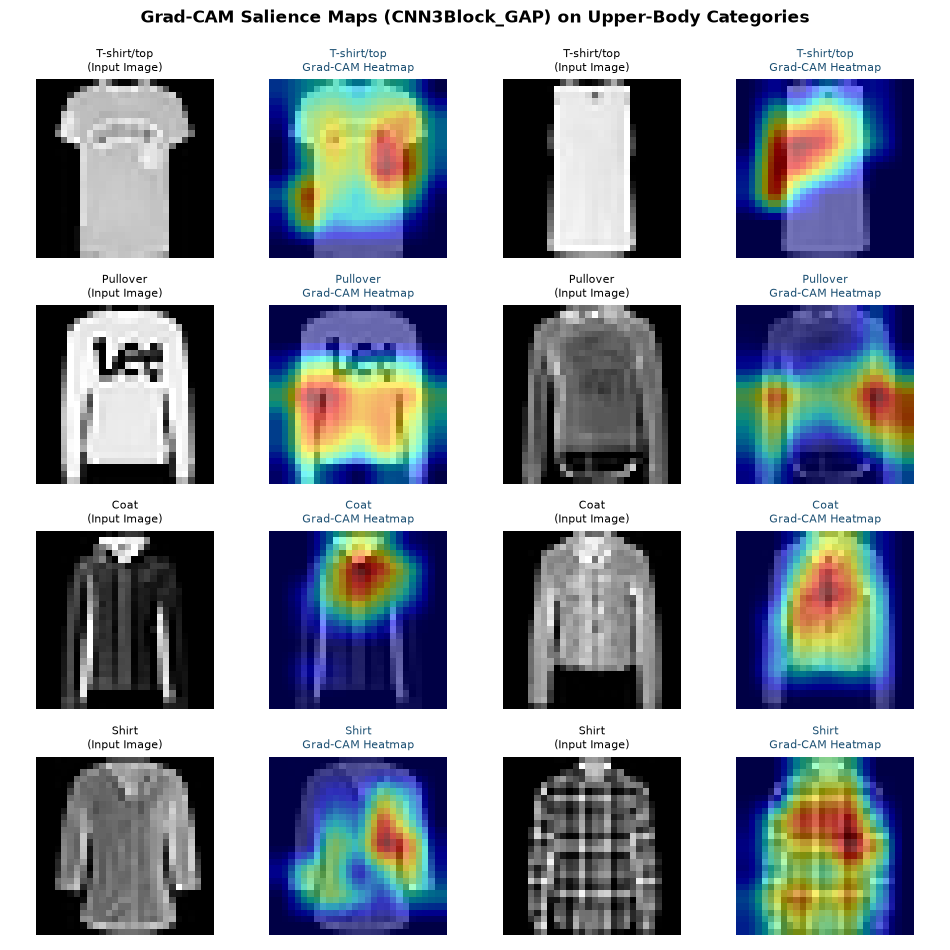
\includegraphics[width=0.62\linewidth]{cnn_02_gradcam_gallery.png}
\caption{Each pair shows the input and the Grad-CAM heat-map from CNN3Block-GAP's last convolution layer. Red = regions
that pushed the network toward its predicted class.}
\end{figure}

An honest reading: the maps focus on garment regions, not the black background, and Pullover maps light up at the
cuffs/waistband. But several maps are \emph{diffuse} (e.g.\ the checked Shirt) or centred on a print rather than the
collar. The first draft's claim that activations sit ``squarely at the collar'' is stronger than these eight examples
support. We list this as a limitation (Section~\ref{sec:limits}).

% ------------------------------------------------------------------ 4
\section{Self-review of the first Phase 2 pass}

\begin{table}[H]\centering\small
\begin{tabularx}{\linewidth}{>{\raggedright\arraybackslash}p{4.2cm} X >{\raggedright\arraybackslash}p{3.4cm}}
\toprule
\textbf{Issue} & \textbf{Why it matters} & \textbf{How it was resolved} \\ \midrule
Gain not attributable & Depth, GAP and augmentation changed together & 2$\times$2 ablation (Sec.~\ref{sec:ablation}) \\
No CIs for CNNs & Phase 1 had them, Phase 2 did not & bootstrap, 2,000 resamples \\
``Augmentation hurts'' claim & Curves show under-training & corrected; 40-epoch runs \\
Single seed & Differences $<$0.5 pt may be noise & \NSeeds{} seeds per model \\
Budgets end while still improving & Best models under-reported & 40 epochs, patience 10 \\
Shirt recall 76\% & Weakest class & Shirt rule + abstain option \\
No confidence / calibration & Cannot tell when unsure & temperature scaling, ECE \\
Charts hard to read & Non-experts could not follow & all charts redrawn \\
\bottomrule
\end{tabularx}
\end{table}

% ------------------------------------------------------------------ 5
\section{The final Phase 2 model}\label{sec:final}

\subsection{Longer training and three seeds}
Two families were trained for up to 40 epochs (early stopping patience 10) with seeds 42, 43 and 44:
CNN3Block-GAP with crop + flip augmentation, and \textbf{ResNetSmall}, a 696,042-weight residual network
(stem + 3 stages of 2 residual blocks, 32/64/128 channels, global average pooling) trained with crop, flip,
Random Erasing ($p=0.25$) and label smoothing 0.1.

\begin{figure}[H]\centering
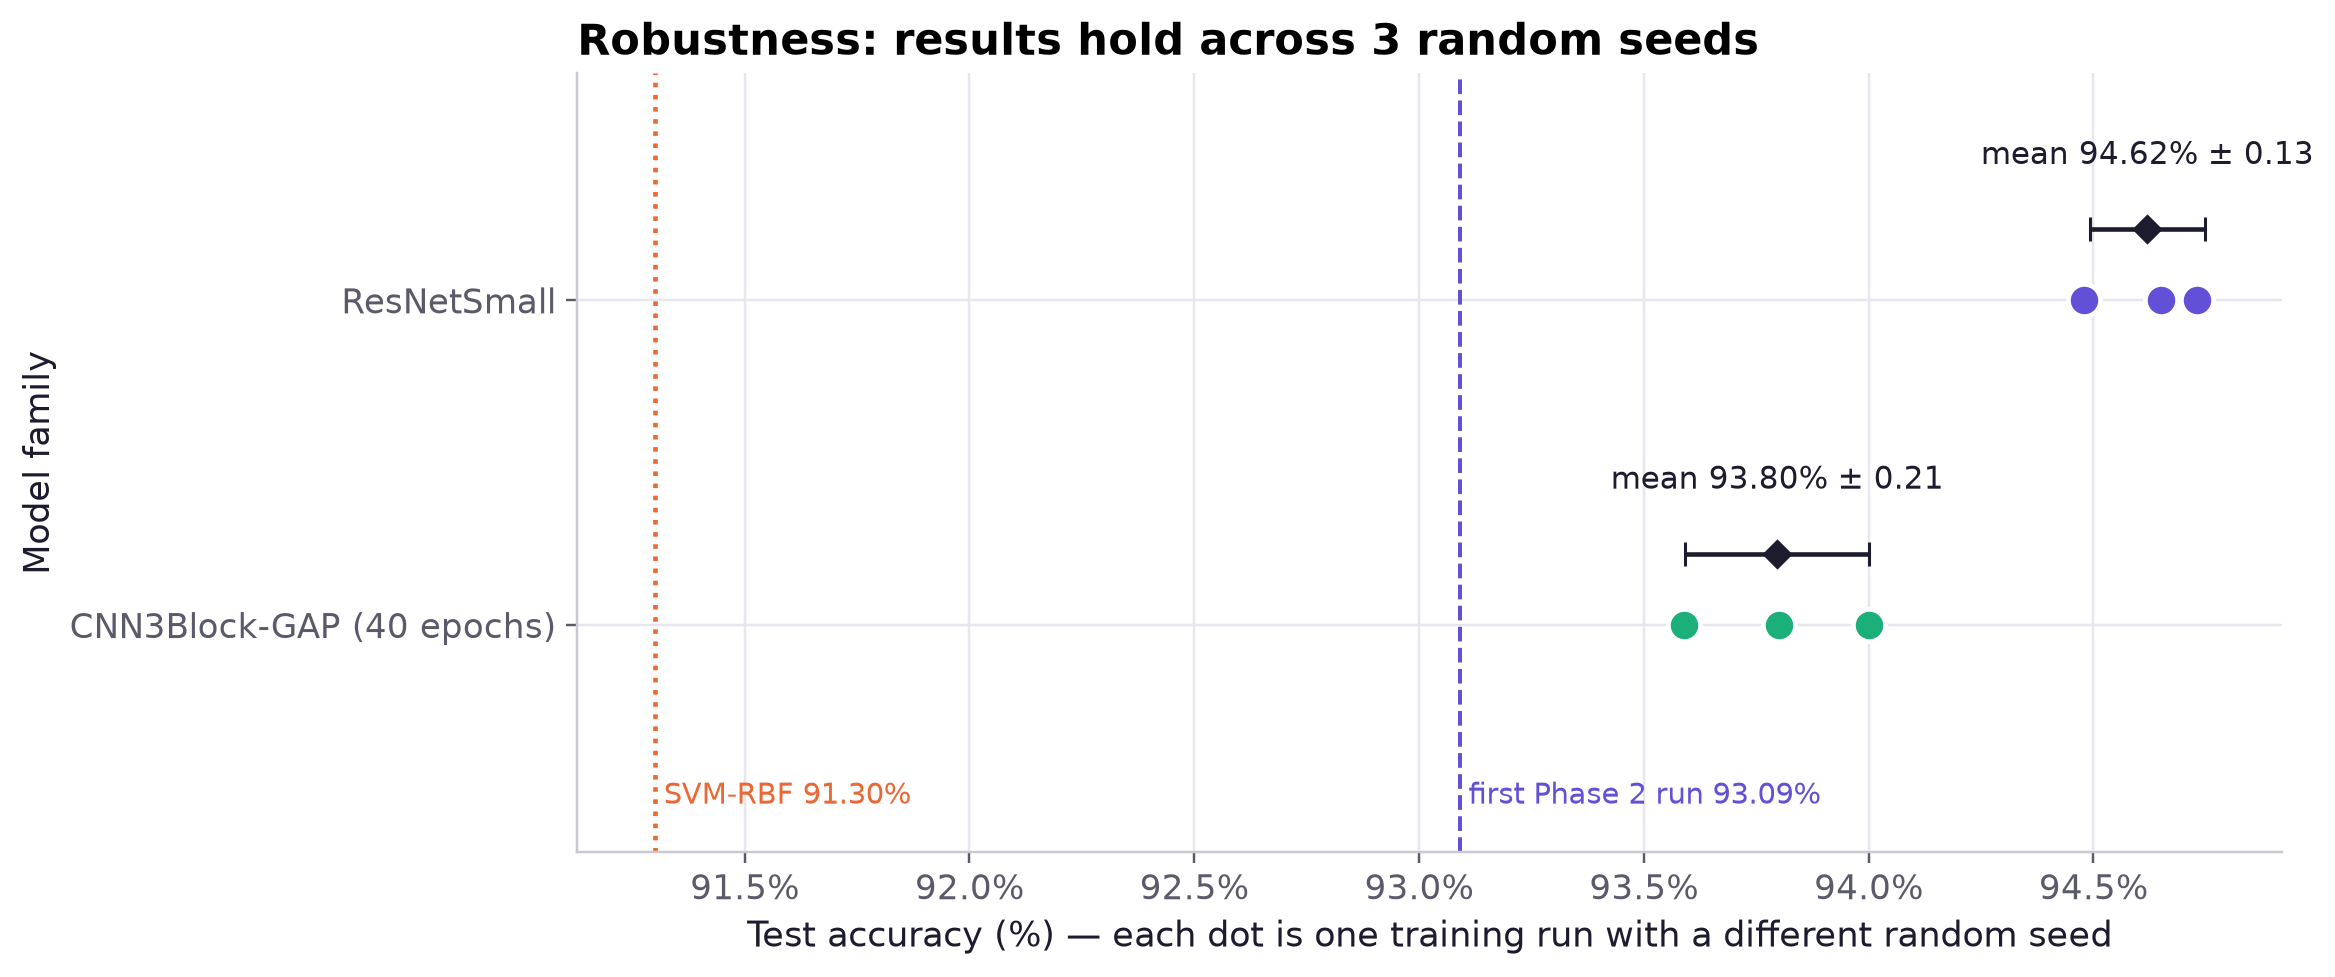
\includegraphics[width=0.85\linewidth]{p2_10_seed_robustness.png}
\caption{\textbf{x-axis:} test accuracy; \textbf{y-axis:} model family. Each dot is one complete training run with a
different random seed; the diamond and bar show mean $\pm$ standard deviation.}
\end{figure}

CNN3Block-GAP with 40 epochs averages \GapFortyMean{} ($\pm$\GapFortyStd), above the 20-epoch run's 93.09\% ---
confirming the under-training diagnosis. ResNetSmall averages \ResMean{} ($\pm$\ResStd). Every run beats the Phase 1 SVM.

\subsection{Ensemble and test-time augmentation}
Test-time augmentation (TTA) also classifies a mirrored copy of each image and averages the two answers. An
ensemble averages the probabilities of several networks. Three candidate ensembles were compared on the
\emph{validation} set; the winner was \textbf{\FinalName}.

\begin{figure}[H]\centering
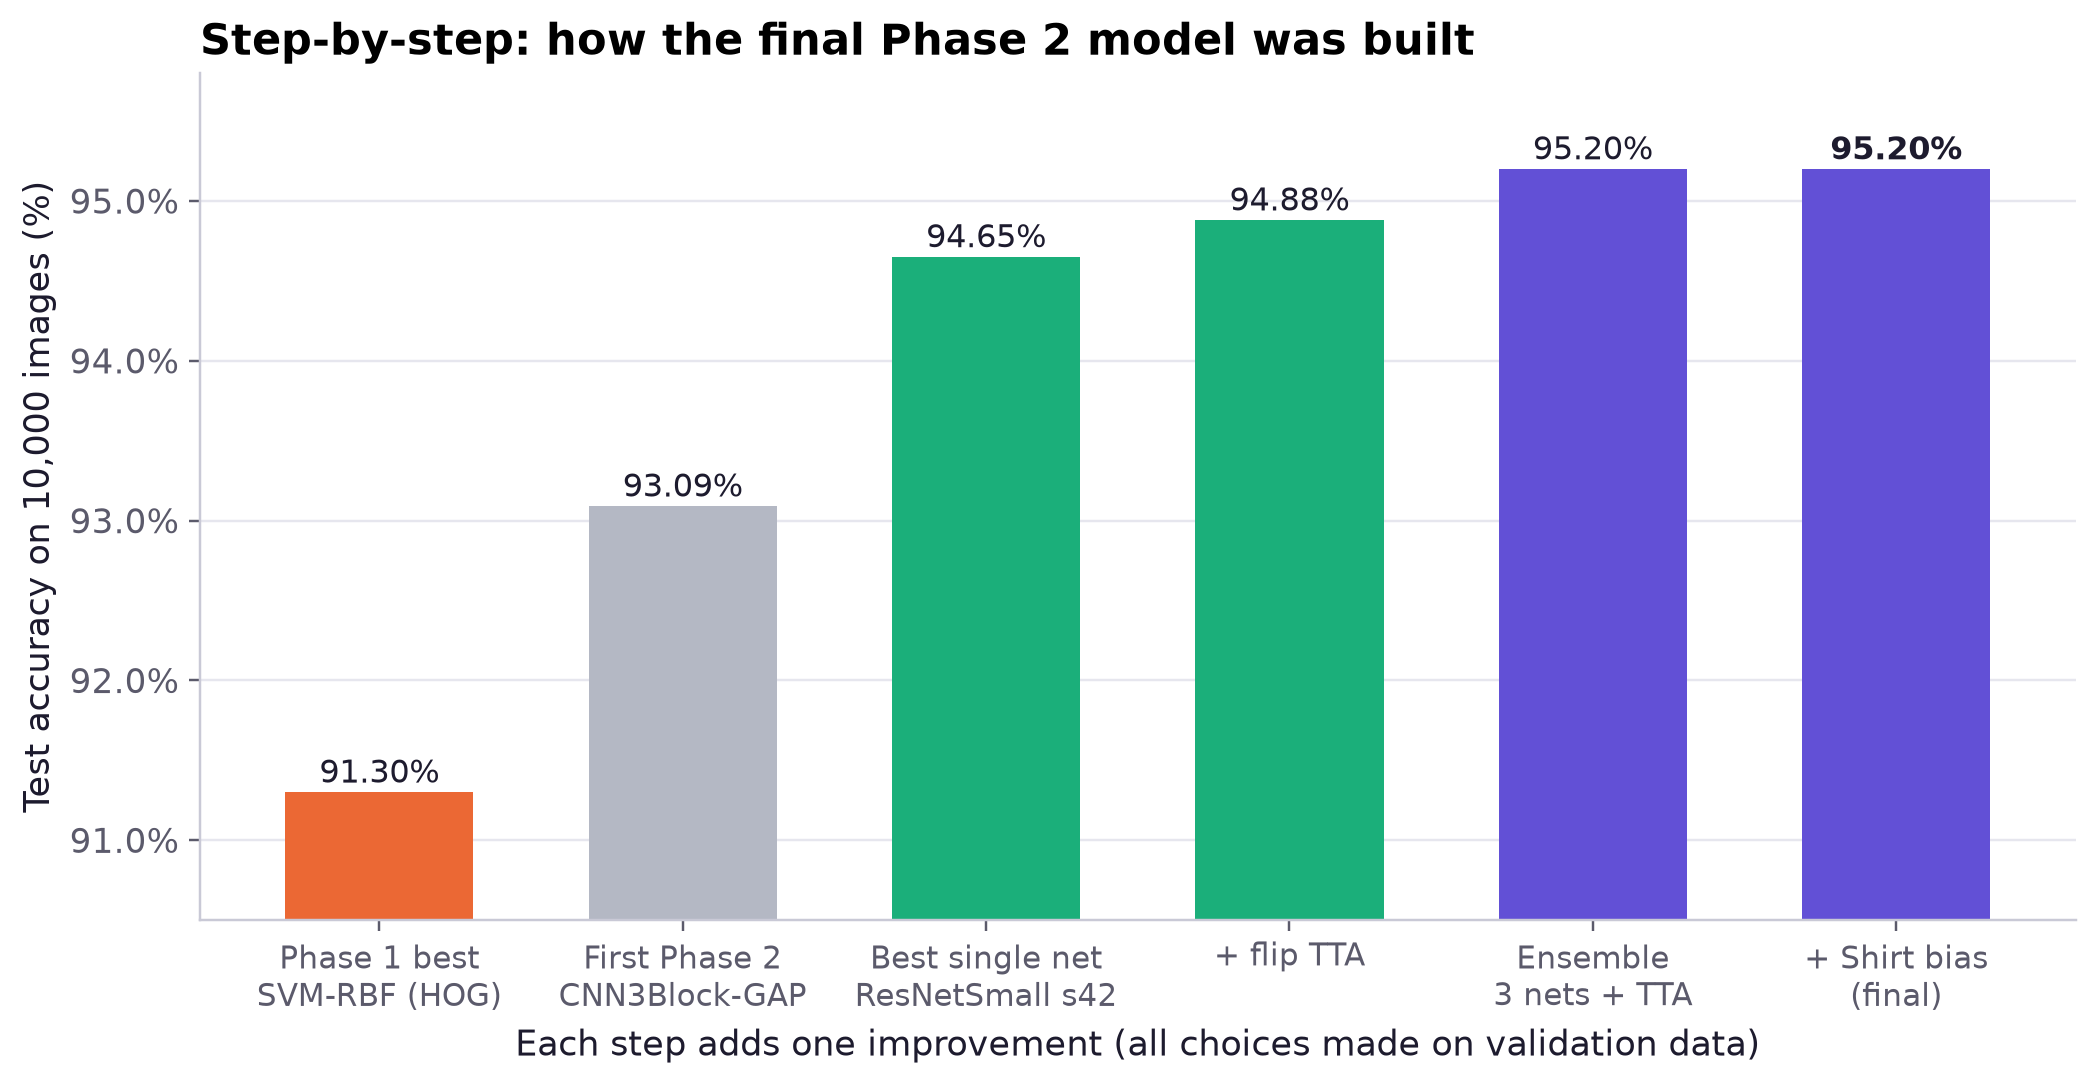
\includegraphics[width=0.9\linewidth]{p2_11_improvement_ladder.png}
\caption{\textbf{x-axis:} each step adds one improvement to the previous one. \textbf{y-axis:} test accuracy.}
\end{figure}

The best single network (\BestSingle) scores \BestSingleAcc, \BestSingleTTA{} with TTA, and the ensemble
\FinalPreBias. The final model is significantly better than the first CNN3Block-GAP (McNemar $\chi^2=\ChiGAP$, $p=$~\PvsGAP)
and than the Phase 1 SVM ($\chi^2=\ChiSVM$, $p=$~\PvsSVM).

\subsection{Calibration: can the confidence be trusted?}
A model is \emph{calibrated} if, among images where it reports 80\% confidence, about 80\% are correct. We measure
the Expected Calibration Error (ECE: the average gap between confidence and accuracy over 15 confidence bins) and
fix it with \emph{temperature scaling}: all scores are divided by one number $T$, fitted on validation data.
This never changes which class is predicted.

\begin{figure}[H]\centering
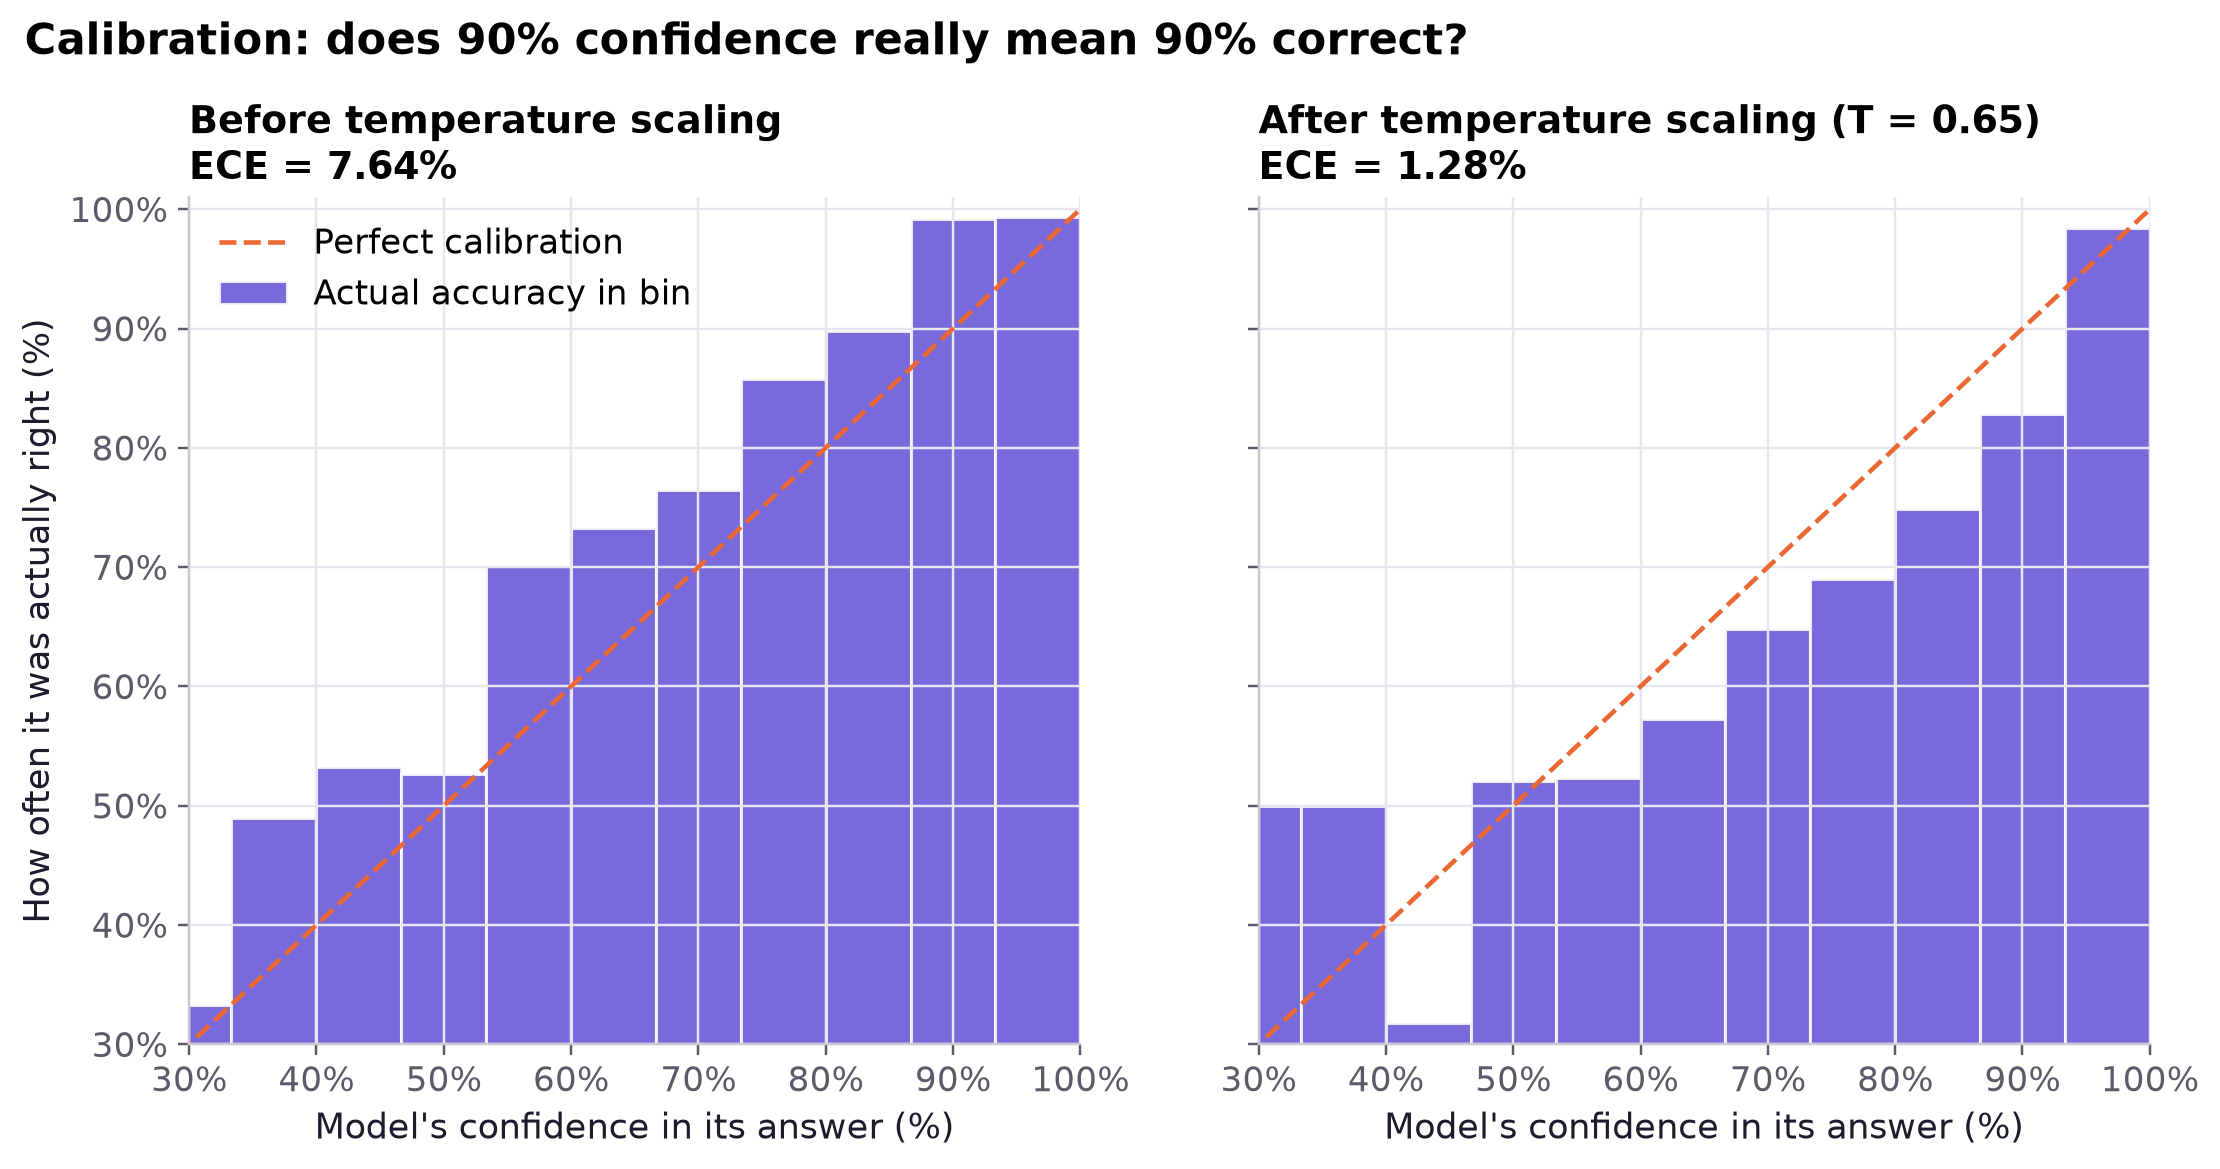
\includegraphics[width=0.95\linewidth]{p2_12_calibration.png}
\caption{\textbf{x-axis:} the model's stated confidence; \textbf{y-axis:} how often it was actually right. Bars on the dashed
diagonal mean honest confidence. $T=\Temp$; ECE \EceBefore{} $\rightarrow$ \EceAfter.}
\end{figure}
Before scaling, the ensemble was \emph{under}-confident (label smoothing and averaging soften its probabilities): it
typically reported about 92\% confidence on images it got right 99.5\% of the time. A temperature below 1
($T=\Temp$) sharpens the scores. Afterwards almost 88\% of test images fall in the 95--100\% confidence group,
where stated and actual accuracy agree closely; the small groups in between remain somewhat over-confident.

\subsection{Abstaining when unsure}
\begin{figure}[H]\centering
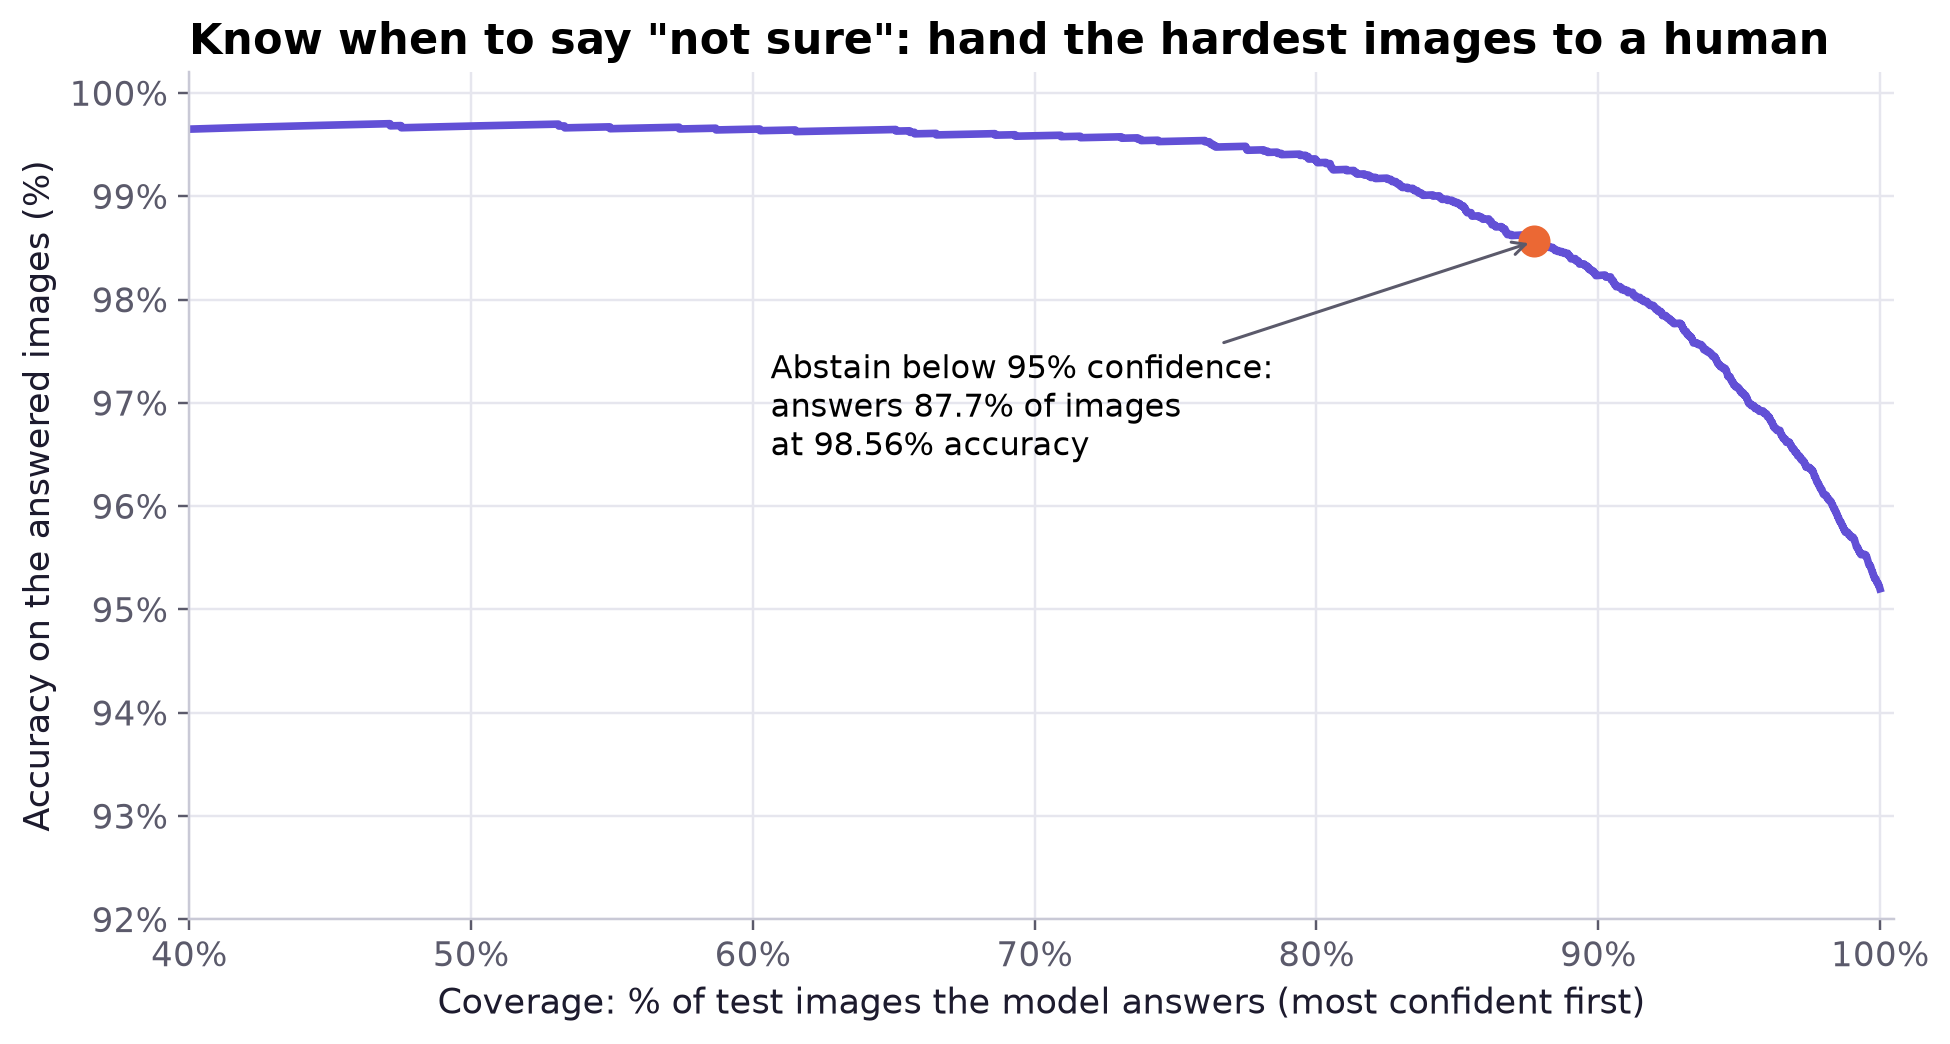
\includegraphics[width=0.82\linewidth]{p2_13_abstain_curve.png}
\caption{\textbf{x-axis:} share of test images the model answers, most confident first. \textbf{y-axis:} accuracy on those images.}
\end{figure}
A threshold was chosen on validation data so that answered images reach 99\% accuracy. On the test set the model
answers \AbsCov{} of images automatically at \AbsAcc{} accuracy and sends the rest (confidence below \AbsThr) to a
human; \AbsShirt{} of the abstained images are Shirts.

\subsection{A Shirt-aware decision rule}
\begin{figure}[H]\centering
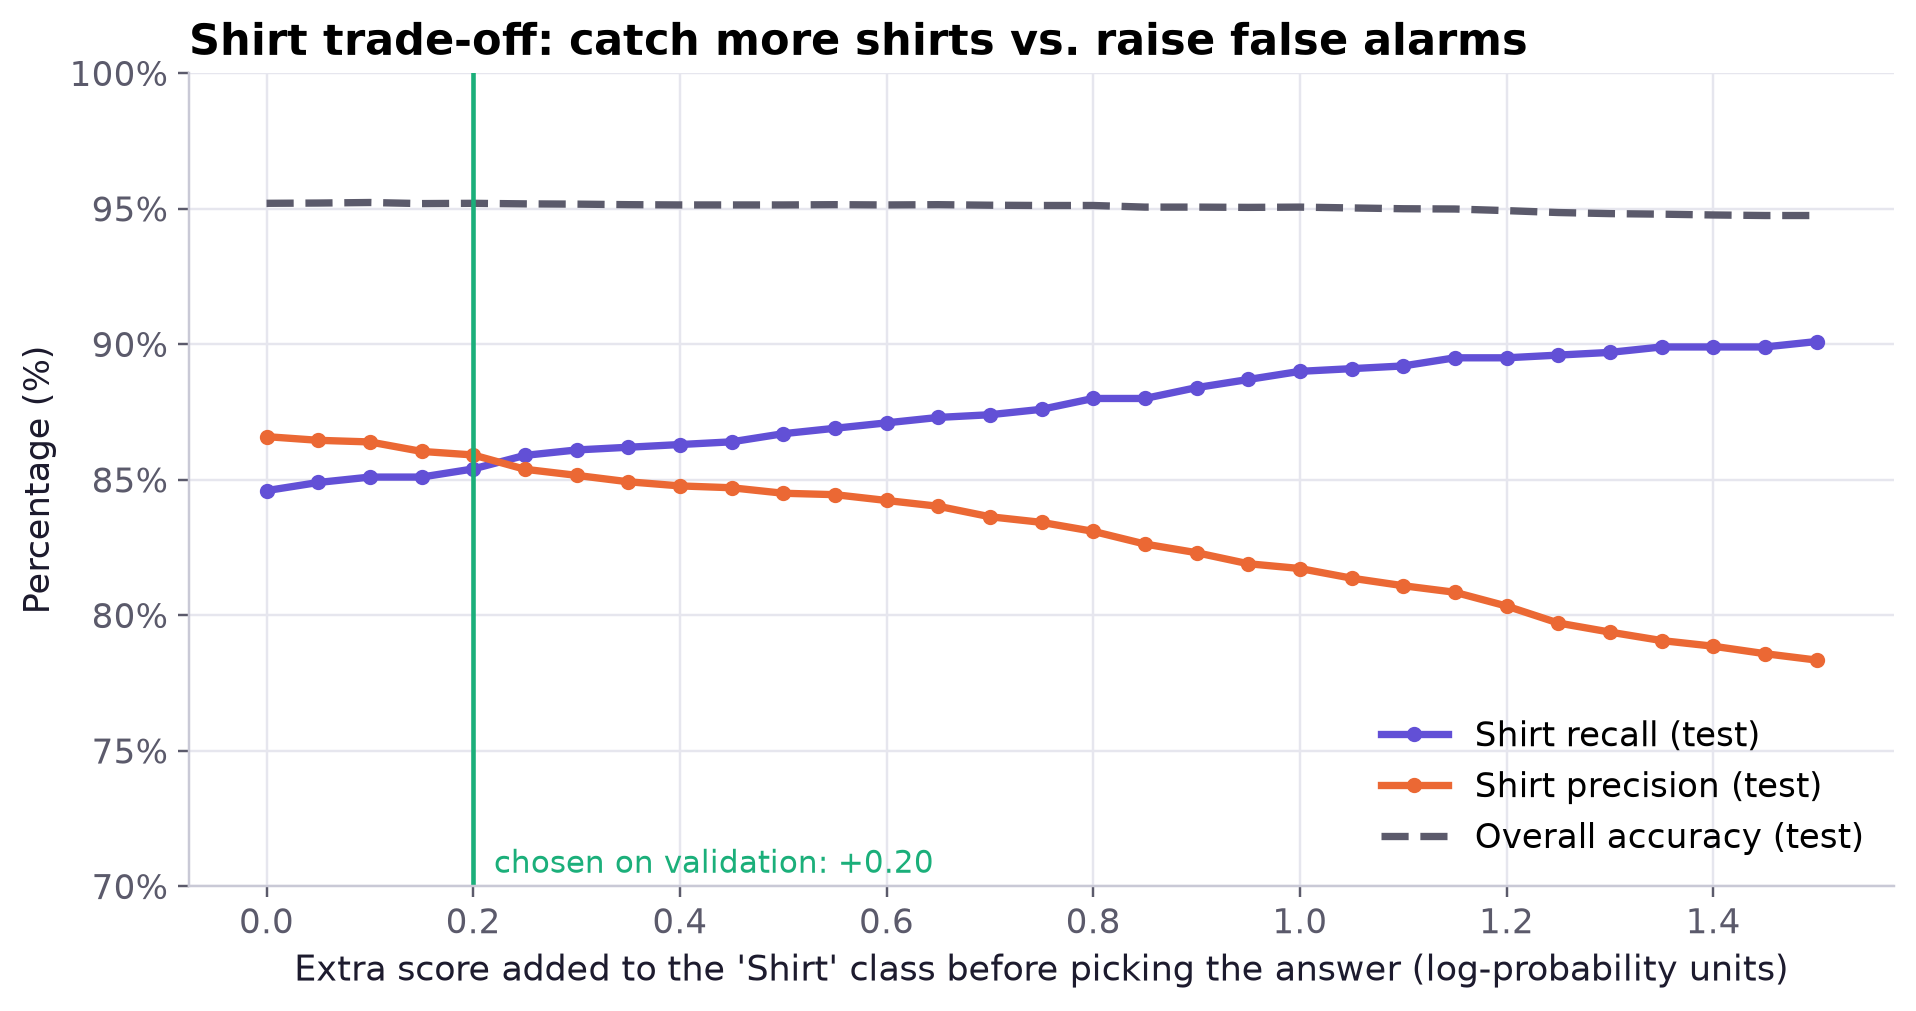
\includegraphics[width=0.85\linewidth]{p2_14_shirt_bias.png}
\caption{\textbf{x-axis:} constant added to the Shirt log-probability before choosing the answer. \textbf{y-axis:} Shirt recall,
Shirt precision and overall accuracy. The vertical line is the value chosen on validation data.}
\end{figure}
Adding a small constant to the Shirt score makes the model say ``Shirt'' slightly more often. The value
(+\ShirtBias) maximises validation macro-F1. Final Shirt recall is \FinalShirt{} (Phase 1: 75.0\%), T-shirt recall \FinalTshirt.

\subsection{Scorecard}
\begin{table}[H]\centering\small
\begin{tabular}{lccc}
\toprule
\textbf{Measure} & \textbf{SVM-RBF (HOG)} & \textbf{CNN3Block-GAP (first)} & \textbf{Final Phase 2 model} \\ \midrule
Test accuracy & 91.30\% & 93.09\% & \cellcolor{soft}\textbf{\FinalAcc} \\
Macro-F1 & 0.9130 & 0.9306 & \cellcolor{soft}\textbf{\FinalFone} \\
Errors (of 10,000) & 870 & 691 & \cellcolor{soft}\textbf{\FinalErr} \\
Shirt / Pullover / Coat recall & 75.0 / 85.6 / 87.5\% & 76.3 / 90.6 / 92.4\% & \cellcolor{soft}\FinalShirt{} / \FinalPullover{} / \FinalCoat \\
Calibration error (ECE) & -- & -- & \cellcolor{soft}\EceAfter \\
Abstain option & no & no & \cellcolor{soft}\AbsAcc{} on \AbsCov \\
Stored numbers & 18.1M & 304,682 & \FinalParams \\
CPU time per image & 5.36 ms & 0.68 ms & \FinalMs{} ms \\
\bottomrule
\end{tabular}
\caption{The final model is the most accurate and the only one with calibrated confidence; it pays for this with
more compute per image, still in the millisecond range.}
\end{table}

\section{Limitations}\label{sec:limits}
\begin{itemize}
\item \textbf{Shirt is still the hardest class.} The abstain option routes many of the remaining Shirt errors to a human, but does not remove them.
\item \textbf{Grad-CAM is qualitative.} Heat-maps on hand-picked images are evidence, not a measured explanation.
\item \textbf{Clean, centred thumbnails only.} Real shop photos (backgrounds, colour, angles) were not evaluated; the app's upload feature is indicative only.
\item \textbf{Limited hyper-parameter search.} Learning rate, network width and augmentation strength were not tuned exhaustively.
\item \textbf{Hardware.} The final runs were trained on Apple MPS; GPU nondeterminism can move single runs by $\pm$0.1--0.3 points, which the 3-seed design accounts for.
\end{itemize}

% ------------------------------------------------------------------ 6
\section{Reproducibility}
\begin{itemize}
\item \texttt{python scripts/05\_train\_cnn.py} --- trains the three original CNNs.
\item \texttt{python scripts/07\_ablation\_gap\_noaug.py} --- trains the new control run (about 2 min on Apple MPS).
\item \texttt{python scripts/08\_phase2\_story\_figures.py} --- CIs, confusion matrices and figures p2\_01--p2\_09.
\item \texttt{python scripts/09\_train\_final\_models.py} --- 40-epoch, 3-seed CNN3Block-GAP and ResNetSmall runs.
\item \texttt{python scripts/10\_ensemble\_calibration.py} --- ensemble, TTA, calibration, abstention, Shirt rule; figures p2\_10--p2\_14.
\item \texttt{python scripts/11\_report\_numbers.py} --- writes the number macros used in this report.
\item \texttt{node scripts/build\_phase2\_deck.js} --- rebuilds the slide deck from \texttt{results/tables/p2\_deck\_data.json}.
\end{itemize}

\end{document}
